\documentclass[preprint,3p]{elsarticle}
%\documentclass[preprint,12pt,authoryear]{elsarticle}

\usepackage{amsmath,amssymb,amsfonts,bbm,bm}%
\usepackage{amsthm}%
\usepackage{mathrsfs}%
\usepackage[dvipsnames]{xcolor}
\biboptions{numbers,sort&compress}
\usepackage{hyperref}
\hypersetup{colorlinks=true}
\usepackage{doi}
%\usepackage{natbib}
\usepackage{booktabs, multirow,threeparttable,tabularx}
\usepackage{algorithm,algorithmicx,algpseudocode}
\usepackage{appendix}
\usepackage{lineno}
\usepackage[belowskip=-1pt,aboveskip=3pt]{caption}
\usepackage[capitalize,nameinlink]{cleveref}

% set the format for notes on in-progress responses
\newcommand\myNote[1]{\textcolor{red!50!black}{(#1})}
\newcommand\myRev[1]{\textcolor{blue!50!black}{(#1)}}
% Revision, copy editing
% NOTE: `\textcolor` does not accept paragraph breaks.
\newcommand{\edit}[1]{\textcolor{red}{#1}} %New/modified text.
\newcommand{\newloc}[1]{\textcolor{blue!80!black}{#1}} %New location without major changes to text.
\newcommand{\tbd}[1]{\textcolor{orange}{#1}} %To be done / dealt with / modified.
% % Disable revision markups: use the following and comment the above.
% \newcommand{\edit}[1]{#1}
% \newcommand{\newloc}[1]{#1}
% \newcommand{\tbd}[1]{#1}

\journal{Computer Methods in Applied Mechanics and Engineering}

\begin{document}

\hypersetup{citecolor = red!50!black ,linkcolor= blue!50!black, urlcolor= blue!50!black}
%\hypersetup{allcolors = black}

\begin{frontmatter}

%% Title, authors and addresses

\title{A novel decoupled approach combining invertible cross-entropy method with Gaussian process modeling for reliability-based design and topology optimization}

% Authors
\author[1]{Thu Van Huynh}
\address[1]{Center of Excellence in Applied Mechanics and Structures, Department of Civil Engineering, Chulalongkorn University, Bangkok 10330, Thailand}

\author[1]{Sawekchai Tangaramvong\corref{cor1}}
\cortext[cor1]{Corresponding author}
\ead{sawekchai.t@chula.ac.th}

\author[2]{Bach Do}
%\ead{bdo3@uh.edu}
\address[2]{Department of Civil and Environmental Engineering, University of Houston, Houston, TX 77204-4003, USA}

\author[3]{Wei Gao}
%\ead{w.gao@unsw.edu.au}
\address[3]{Centre for Infrastructure Engineering and Safety, School of Civil and Environmental Engineering, The University of New South Wales, Sydney, NSW 2052, Australia}

\begin{abstract}
%% Text of abstract
{Design optimization considering the presence of uncertainties in parameters poses an extremely challenging problem. The source of difficulties comes with reliability-based formulations, where addressing the probabilistic problem exhausts the large computing efforts for failure estimations of the structure violating limit-state functions (LSFs). This paper proposes a novel decoupled approach for effectively solving reliability-based design optimization (RBDO) problems, namely an invertible cross-entropy (iCE) method advantageously combined with a Gaussian process regression (GPR) model, termed as iCE-GPR. The GPR model is applied to approximate the spectrum of LSFs under random parameters. Furthermore, to enhance the accurate prediction of the system failure probability, an active learning process is applied to systematically refine the GPR model by adding new learning points in the region with the largest uncertainty and high-reliability sensitivity through the maximization of an expected feasibility function (EFF). Based on the updated GPR model, the failure probability is estimated by a cost-effective cross-entropy (CE) method without any calls to the actual performance function. To perform the decoupling optimization process with the reliability analysis, the novel iCE, based on the CE method, is developed to update the most probable point (MPP) assigned for the next deterministic optimization process in determining the new optimal design. The method iteratively performs the deterministic optimization process based on the MPP underpinning LSFs sequentially updated by the active learning process. The proposed iCE-GPR method fast-converges the optimal design and significantly alleviates computational burdens associated with reliability analyses. The proposed method is also applied to solve a reliability-based topology optimization (RBTO) problem. Four numerical examples for both the RBDO and RBTO problems are provided to illustrate efficiency and robustness of the proposed iCE-GPR method. 
}
\end{abstract}

%%Graphical abstract
%\begin{graphicalabstract}
%\includegraphics{grabs}
%\end{graphicalabstract}

%%Research highlights
\begin{highlights}
\item A novel RBDO approach combines deterministic design optimization with GPR model-assisted cross-entropy method.
\item Active learning reliability analyses performed on the GPR model improve the accuracy of failure probability estimates. 
\item Uncertainty in limit-state functions for processing optimization is captured by most probable points.
\item Invertible cross-entropy method quickly estimates the most probable points.
%\item Examples illustrate the efficiency and robustness of the proposed iCE-GPR method in solving both RBDO and RBTO problems.
\end{highlights}

\begin{keyword}
SIMP \sep Gaussian process regression \sep Comprehensive learning PSO \sep Active learning \sep Invertible cross-entropy method
%% keywords here, in the form: keyword \sep keyword

%% PACS codes here, in the form: \PACS code \sep code

%% MSC codes here, in the form: \MSC code \sep code
%% or \MSC[2008] code \sep code (2000 is the default)

\end{keyword}

\end{frontmatter}

\begin{linenumbers}

\clearpage

%% main text
\section{Introduction}
\label{sec1}
Design optimization has been widely used to improve system performance in various fields of engineering applications. Traditionally, engineering design optimization is formulated as deterministic design optimization (DDO). However, the optimal solution obtained by the DDO may be unreliable due to negligence of various aleatory and epistemic uncertainties that exist inherently in the structures \cite{tangaramvong2015, Do2014} under practical engineering design (e.g., structural dimensions, material properties, loading, manufacturing tolerance, incomplete knowledge, and operating conditions). To guarantee that structures perform in a highly safe manner with ultimate safety condition levels in comparison with the unreliable DDO, a reliability-based design optimization (RBDO) approach \cite{Frangopol2003, Schueller2008, Valdebenito2010, Aoues2010, Moustapha2019, meng2023} has been employed to simultaneously address the performance and reliability of the structure in a probabilistic way. In addition, the RBDO has been extended to the area of topology optimization, resulting in what is known as reliability-based topology optimization (RBTO). This approach, as studied in \cite{TAUZOWSKI2021, kharmanda2004, MOVAHEDIRAD2023, KESHTEGAR2023, VISHWANATHAN2019, LEI2023, MENG2020, YIN2018}, addresses various sources of uncertainties in engineering structures. In essence, both the RBDO and RBTO problems take into account the probabilistic constraints of parameter uncertainty, and therefore its safety under every failure scenario is measured explicitly and rigorously. 

Conventionally, the key difficulty of RBDO is concerned with the coupling of the optimization process and reliability analysis. Various RBDO approaches have been developed to make the RBDO problem computationally tractable and possible to converge to a reliable solution. Depending on how the probability constraints are handled during the optimization process, the literature categorizes RBDO into three main types, including double-loop \cite{Zhang2021, youn2003, NIKOLAIDIS1988, KESHTEGAR2018a, keshtegar2018b, RASHKI2012, Yang2020, Hao2019}, single-loop \cite{Mansour2016, Jiang2017, Meng2019, Wauters2021, Yang2021, YANG2022, MENG2019a, liang2007, MENG2015, jeong2017}, and decoupling approaches \cite{Du2004, Goswami2019, Li2016, FAES2020, Li2020, ZHANG2021a, zhang2021b, jiang2020, hamza2022, chen2018, SafaeianHamzehkolaei2016, zheng2023}. 

The traditional double-loop approach employs a nested loop in which an outer deterministic optimization loop and an inner loop handling the probabilistic constraints. In reliability analysis, the failure probabilities can be estimated using conventional sampling methods such as the Monte-Carlo simulation (MCS) \cite{RASHKI2012}, or approximation methods including the first-order reliability analysis (FORM) or second-order reliability analysis (SORM), which comprise the reliability index approach (RIA) \cite{Zhang2021, youn2003, NIKOLAIDIS1988, Yang2020} and performance measure approach (PMA) \cite{KESHTEGAR2018a, keshtegar2018b, Hao2019}. Unfortunately, the double-loop approach often offers poor performance and accuracy of the first- and second-order reliability methods due to the highly nonlinear LSFs, or the huge computational cost of the crude MCS due to the curse of dimensionality. Even when using advanced sampling methods such as importance sampling (IS) \cite{CHAUDHURI2020} and subset simulation (SS) \cite{li2016a} whose cost is relatively small compared to the crude MCS, the overall cost of such methods is still prohibitively high. 

The single-loop approach has been suggested to overcome the mentioned drawbacks of the double-loop approach by replacing all probabilistic constraints with the equivalent deterministic constraints. In the early studies, some single-loop approaches based on Karush–Kuhn–Tucker optimality conditions were used to achieve high convergence speed \cite{liang2007}. Although the single-loop formulation can avoid direct calculation of the failure probability, it may encounter the non-convergence phenomena for strongly nonlinear problems \cite{MENG2019a}. To enhance the global convergence, several improved versions have been proposed recently, such as the single-loop single-vector method \cite{jeong2017}, hybrid single-loop approach \cite{Jiang2017, Yang2021}, enhanced advanced mean value method  \cite{yang2020a}, and conjugate gradient and chaotic control methods \cite{yang2020a, MENG2019a, MENG2015}. 

To avoid the computational burden of the double-loop approach and the non-convergence of the single-loop approach, the so-called decoupled approach has been proposed \cite{Du2004, Aoues2010}, in which the nested probabilistic loop is transformed into a sequence of deterministic optimizations and reliability analysis. It means that the decoupled approach implements the reliability analysis only once after deterministic optimal design from the outer loop is achieved. As a result, the approach can significantly reduce the number of reliability analyses, which account for a majority of the total computational costs in the RBDO. Normally, the decoupled methods use the conception of the most probable point (MPP) of the random variable to perform reliability analysis, one of the most well-known methods is sequential optimization and reliability assessment (SORA) \cite{Du2004, Li2020, jiang2020}. Based on the SORA, several decoupling strategies have been developed, including the optimal shifting vector \cite{Goswami2019, ZHANG2021a, SafaeianHamzehkolaei2016, zheng2023}, probabilistic feasible region \cite{chen2018}, and other up-to-date methods \cite{Li2016, zhang2021b, hamza2022}. In summary, the decoupled methods have exhibited relatively higher efficiency compared to the other approaches.

In recent years, machine learning-based surrogate models have gained a large amount of attention. The surrogate model aims to construct a cheap approximation model through the design of experiments to replace a computationally expensive model (e.g., the implicit performance functions in the RBDO problem). This research direction emerges from the fact that structural analyses implicit within a finite element analysis (FEA) program are less advantageous to processing optimization as well as reliability analysis. Various well-known surrogate models have been employed for engineering problems such as artificial neural networks \cite{Lehky2018, Papadrakakis2002, LI2022a}, radial basis function \cite{Jing2019, Shang2021}, and support vector machine \cite{Moustapha2019, Cheng2020, liu2017}. One of the most commonly used surrogate models in this direction is the Gaussian process regression (GPR) \cite{Yang2021, YANG2022, Ni2020, Su2017, Li2019} as it can offer a flexible application to any sophisticated functions with a high-level accuracy of predictions. The GPR model provides the response predictions in unexplored areas, along with the local variance of the prediction, that is, the model uncertainty of surrogates. Moreover, the active learning process governed by the GPR \cite{MOUSTAPHA2022, XIAO2020, WANG2024, WEI2023} has been successfully applied for solving many complex RBDO problems due to its flexibility in using adaptive samples in the specific region under the required accuracy. The machine learning-based surrogate methods can be developed as a flexible and nonlinear model that is used for nonlinear predictions of the failure domain in the optimization level under uncertainties. The accuracy of the machine learning approaches is the main challenge for developing a model applied in RBDO. The reviews of the state-of-the-art machine learning-based surrogate models for the solutions of structural reliability analysis and RBDO problem can be seen in \cite{Moustapha2019, SaraygordAfshari2022, TEIXEIRA2021, CUI2019}. Although substantial efforts have been made to enhance the computational efficiency and robustness of reliability analysis, several challenges still persist in situations when large-scale problems with many design and random variables under various types (integer-discrete-continuous) or strong non-linearities in the probabilistic constraint functions are considered. This context leaves plenty of room for developing more powerful methods, which will effectively improve the ability to solve many complex engineering problems and hence greatly increase the practical use of the RBDO. 

In light of the aforementioned background, incorporating the machine learning-based surrogate models into the decoupling approach clearly offers the computational benefit in solving the RBDO problems. Three critical aspects needed to quickly obtain a reliable solution to practical scale problems with modest computing efforts are: (1) the robustness of optimization algorithms for solving the deterministic optimization problems, (2) the construction of the efficient surrogate model, and (3) the MPP update scheme. In order to reach these goals, this paper proposes an efficient decoupled RBDO approach named iCE-GPR, which combines a GPR model with an invertible cross-entropy (iCE) method. To start off with the iCE-GPR, the DDO is implemented by using a comprehensive learning particle swarm optimization (CLPSO) for structural optimization or a solid isotropic material with penalization (SIMP) for topology optimization. Then, the GPR as a probabilistic surrogate model is constructed to presume the spectrum of the actual performance function of interest under the random parameters, thereby enabling the cost-efficient cross-entropy (CE) method to quickly estimate the failure probability associated with the optimal design corresponding to the current MPP without any calls to the actual performance function. To fully define the failure surface of the performance function, especially the border distinguishing the failure region from the safe one, the GPR model is strategically refined through an active learning process by adding the new learning points to the region with the largest uncertainty and high-reliability sensitivity that is further transferred to maximizing a so-called expected feasibility function (EFF). Here, the CLPSO is adopted to optimize both the GPR hyperparameters and the active learning function EFF. Remarkably, the novel iCE method is developed to identify a new MPP for the next decoupling formulation in finding the new optimal design. This optimization process is carried out in a sequential way until the failure probability associated with the optimal design by the deterministic optimization reaches the allowable threshold. 

\section{Proposed decoupling RBDO and RBTO method}
\label{sec2}

\subsection{Problem formulation}\label{SUBSEC:21}
Both RBDO and RBTO problems considered in this work minimize an objective function $\mathcal{C}(\textbf{s})$ under certain deterministic and probabilistic constraints. A general form of these problems is as follows \cite{VANHUYNH2023}:
% Equation 1
\begin{equation}
    \begin{aligned}
        \underset{\textbf{s}}{\text{minimize}} \quad & \mathcal{C}(\textbf{s})\\
        \text{subject to} \quad &
        \mathbb{P}\bigl[\mathcal{G}_i(\textbf{s},\textbf{x})-\bar{\xi}_i \geq 0\bigr]-\mathcal{P}_{\text{a},i} \leq 0 \,; \forall i \in \{1,\dots,I\},\\
        & \mathcal{H}_j(\textbf{s}) \leq 0 \,; \forall j \in \{1,\dots,J\},\\
        &\textbf{s} \in [\textbf{s}_\text{L},\textbf{s}_\text{U}],
    \end{aligned}
    \label{EQ:1}
\end{equation}
where $\textbf{s}\in\mathbb{R}^{n_\text{s}}$ denotes the vector of design variables that consist of size parameters of a size optimization problem or element’s relative densities of a topology optimization problem.
$\textbf{s}_\text{L}$ and $\textbf{s}_\text{U}$ are the lower and upper bounds of $\textbf{s}$, respectively.
$\textbf{x}\in\mathbb{R}^{n_\text{x}}$ is a vector of random parameters supported on a probability space, in which $\Omega$ and the joint probability density function (PDF) $p(\textbf{x})$ are the random space and the probability measure, respectively.  $\mathcal{H}_j(\textbf{s}): \mathbb{R}^{n_\text{s}} \mapsto \mathbb{R}$ are the
deterministic constraint functions. $\mathcal{G}_i(\textbf{s},\textbf{x})$
and $\mathcal{G}_i(\textbf{s},\textbf{x})-\bar{\xi}_i: \mathbb{R}^{n_\text{s}} \times
\mathbb{R}^{n_\text{x}} \mapsto \mathbb{R}$ are the performance function and the corresponding limit state function (LSF) with $\bar{\xi}_i$ denoting a constant threshold for $\mathcal{G}_i(\textbf{s},\textbf{x})$ values.
Problem~(\ref{EQ:1}) assumes that the constraint functions $\mathcal{G}_i(\textbf{s},\textbf{x})$ are conditionally independent given the design variable vector $\textbf{s}$.
If the response value exceeds its threshold, the structure is then determined non-functional. Hence, the domain $\mathcal{F}=
\left\{\textbf{x} \in \Omega|\mathcal{G}_i(\textbf{s},\textbf{x})-\bar{\xi}_i
\geq 0\right\}$ is considered a failure domain for a specific $\textbf{s}$. This domain corresponds to the failure probability $\mathcal{P}_{\text{f}, i} = \mathbb{P}\bigl[\mathcal{G}_i(\textbf{s},\textbf{x})-\bar{\xi}_i\geq 0\bigr] = \idotsint_\mathcal{F} p(\textbf{x})\mathrm{d}\textbf{x}$, where $\mathbb{P}[\cdot]$ denotes the probability operator. $\mathcal{P}_{\text{a},i}$ is the allowable threshold of $\mathcal{P}_{\text{f},i}$. Generally, estimating the failure probabilities $\mathcal{P}_{\text{f}, i}$ is challenging as it is an intrinsic NP-hard problem \cite{VANHUYNH2023, Do2021b}. 

An idea for addressing problem~(\ref{EQ:1}) is to solve a series of its deterministic counterparts.
Such deterministic problems are formulated for approximate most probable points $\textbf{x}_\text{MPP}$ at which the maximum likelihood of failure is likely to occur given several observations of the uncertain performance functions.
The general formulation of these deterministic problems is  
% Equation 1B
\begin{equation}
	\begin{aligned}
		\underset{\textbf{s}}{\text{minimize}} \quad & \mathcal{C}(\textbf{s})\\
		\text{subject to} \quad &
		\mathcal{G}_i(\textbf{s},\textbf{x}_\text{MPP})-\bar{\xi}_i \leq 0 \,; \forall i \in \{1,\dots,I\},\\
		& \mathcal{H}_j(\textbf{s}) \leq 0 \,; \forall j \in \{1,\dots,J\},\\
		&\textbf{s} \in [\textbf{s}_\text{L},\textbf{s}_\text{U}].
	\end{aligned}
	\label{EQ:1B}
\end{equation}

\subsection{Deterministic topology optimization }\label{SUBSEC:22}
In this work, deterministic topology optimization employs a solid isotropic material with penalization (SIMP) \cite{andreassen2011, sigmund2001} method to find the optimal material distribution within the designated design domain while adhering to specified constraints. An objective is to minimize the total material volume $\mathcal{C}(\textbf{s}) = \sum_{e=1}^{n_\text{s}}{s_{e}}$, where $\textbf{s}\in\mathbb{R}^{n_\text{s}} = \left\{{s_{e}}\in \left[ 0,1 \right]|\forall e\in\{1,\dots,{n_\text{s}}\right\}$ denotes relative material densities, with a binary encoding (0 or 1) indicating the material absence or presence, and $n_\text{s}$ represents the total number of elements within the discretized design domain. The constraint functions $\mathcal{G}_i(\textbf{s},\textbf{x})$ and $\mathcal{H}_j(\textbf{s})$ define the structural compliance, displacement, or other structural metrics. Within the SIMP framework, the interpolation of Young’s modulus for the $e$-th element follows the following approach \cite{andreassen2011}:
% Equation 2
\begin{equation}
E_e=E_{\min}+s_e^p\left(E_0-E_{\min}\right), 
\label{EQ:2}
\end{equation}
where $E_0$ is the elastic modulus of the solid material, $E_{\min}$ is the very small elastic modulus of the void material (e.g., $E_{\min} = 10^{-9}$) assigned to avoid singularities of the finite element stiffness matrix, and $p$ is the penalization factor (typically $p$ = 3). The Young’s modulus values for all elements collectively form the global stiffness matrix ${\bf K(s)}$  governing the equilibrium equation ${\bf K(s)}{\bf u}={\bf F}$, where ${\bf u}$ and ${\bf F}$ are the nodal displacement and load vectors, respectively.
Given the substantial number of design variables inherent in topology optimization problems, the optimality criteria  (OC) method \cite{andreassen2011,zhou2021} is employed for updating the design variables $\textbf{s}$.
This OC updating the scheme reads
% Equation 3
\begin{equation}
s_e^\mathrm{new}=\begin{cases}{\mathrm{max}\left(0,s_{e}-m\right)} & {{\mathrm{if}\ \ s_{e}\mathcal{B}_{e}^{\eta}\leq\mathrm{max}\left(0,s_{e}-m\right)}},\\
{\mathrm{min}\left(1,s_{e}+m\right)} & {{\mathrm{if}\ \ s_{e}\mathcal{B}_{e}^{\eta}\geq\mathrm{min}\left(1,s_{e}-m\right)}}, \\
s_{e}\mathcal{B}_{e}^{\eta} & {{\mathrm{otherwise}}},\end{cases}
\label{EQ:3}
\end{equation}
where ${m}$ is a positive moving-limit set at 0.2, ${\eta}$ is a numerical damping coefficient (empirically ${\eta} =0.5$), and ${\mathcal{B}_{e}}$ is obtained from the Karush-Kuhn-Tucker optimality condition, which is
% Equation 4
\begin{equation}
\mathcal{B}_{e}=-\frac{\partial{\mathcal{C}}}{\partial{s_{e}}}\left(\lambda\frac{\partial{\mathcal{G}}}{\partial{s_{e}}}\right)^{-1}
\label{EQ:4}.
\end{equation}
Here, $\lambda$ is the Lagrangian multiplier computed through a bisection algorithm. The objective and constraint sensitivities are computed as \cite{zhou2021}
% Equation 5
\begin{equation}
\frac{\partial{\mathcal{C}}}{\partial{s_{e}}} = 1,
\label{EQ:5}
\end{equation}
% Equation 6
\begin{equation}
\frac{\partial{\mathcal{G}}}{\partial{s_{e}}} = -ps_e^{p-1}\left(E_0-E_\mathrm{min}\right){{\bf u}_e^{T}}{{\bf K}_e}{{\bf u}_e},
\label{EQ:6}
\end{equation}
where ${\bf K}_e$ is the element stiffness matrix and ${\bf u}_e$ is the element displacement. To mitigate potential numerical instabilities, such as mesh dependency and the occurrence of checkerboard patterns, a modified sensitivity filter \cite{andreassen2011} is implemented:
% Equation 7
\begin{equation}
\frac{\partial\widetilde{\mathcal{G}}\left({\bf s}\right)}{\partial s_{e}}=\frac{\displaystyle\sum_{n\in\mathcal{S}}\mathcal{W}_{e,n}s_{n}\frac{\partial{\mathcal{G}\left(s\right)}}{\partial{s_{n}}}}{\mathrm{max}\displaystyle\left(\gamma,s_{e}\right)\sum_{n\in S}\mathcal{W}_{e,n}}.
\label{EQ:7}
\end{equation}
Here, ${\mathcal{S}}$ is the set of elements $n$ for which the center-to-center distance $\Theta\left({e, n}\right)$ to element $e$ is smaller than the filter radius $r_\mathrm{min}$. $\gamma$ is a small positive number to prevent division by zero, e.g., $\gamma = 10^{-3}$. $\mathcal{W}_{e,n}$ is a weighting function defined as
% Equation 8
\begin{equation}
\mathcal{W}_{e,n} = {\mathrm{max}\left(0, r_\mathrm{min}-\Theta\left({e, n}\right)\right)}.
\label{EQ:8}
\end{equation}
The weighting function exhibits a linear decay with distance from element $n$. Consequently, instead of employing the original sensitivities as presented in \cref{EQ:6}, the OC updating scheme in \cref{EQ:4} utilizes the modified sensitivities outlined in \cref{EQ:7}. 

\subsection{Surrogate-assisted cross-entropy method for reliability analysis}\label{SUBSEC:23}
The primary objective of this work is to reduce the tremendous computational cost associated with conducting the requisite reliability analysis for solving problem~(\ref{EQ:1}).
This is achieved through the development of GPR models, constructed from an initial training set $\mathcal{D}$, to serve as surrogates for the performance functions $\mathcal{G}_i\left(\textbf{s},\textbf{x}\right)$; see Appendix for details.
More specifically, let $\widehat{\mathcal{G}}(\textbf{x})\sim\mathcal{N}\bigl(\mu_{\widehat{\mathcal{G}}}(\textbf{x}),\sigma_{\widehat{\mathcal{G}}}^2(\textbf{x})\bigr)$ represent the Gaussian distribution of the GPR predictive posterior for $\mathcal{G}\left(\textbf{s},\textbf{x}\right)$ at a particular design variable vector $\textbf{s}\in\mathbb{R}^{n_\text{s}}$, where $\mu_{\widehat{\mathcal{G}}}(\textbf{x})$ and $\sigma_{\widehat{\mathcal{G}}}^2(\textbf{x})$ are the predictive mean and predictive variance of the prediction, respectively.
For simplicity, $\mathcal{G}\left(\textbf{s},\textbf{x}\right)$ is henceforth denoted as $\mathcal{G}\left(\textbf{x}\right)$.
The GPR model $\widehat{\mathcal{G}}(\textbf{x})$ facilitates the estimation of the unbiased failure probability $\mathcal{P}_{\text{f}}$ for the design variable $\textbf{s}$ in problem~(\ref{EQ:1}) by using the following crude MCS:
% Equation 9
\begin{equation}
    \mathcal{P}_\text{f} \approx \int_\Omega \mathbb{I}\bigr[\mu_{\widehat{\mathcal{G}}}(\textbf{x}) - \bar\xi\bigl]p(\textbf{x})\mathrm{d}\textbf{x} \approx \frac{1}{N_\text{MCS}}\displaystyle\sum_{k=1}^{N_\text{MCS}} \mathbb{I}\bigr[\mu_{\widehat{\mathcal{G}}}(\textbf{x}_k) - \bar\xi\bigl],
\label{EQ:9}
\end{equation}
where $\textbf {x}_k$, $k\in\{1,\dots,N_\mathrm{MCS}\}$, denote samples randomly generated over $\Omega$, and the indicator function 
$\mathbb{I}[\cdot]$ reads
% Equation 10
\begin{equation}
    \mathbb{I}\bigr[\mu_{\widehat{\mathcal{G}}}(\textbf{x}_k) - \bar\xi\bigl] =
    \begin{cases}
        1  & \quad \text{if } \mu_{\widehat{\mathcal{G}}}(\textbf{x}_k) - \bar\xi \geq 0,\\
        0  & \quad \text{otherwise}.
    \end{cases}
\label{EQ:10}
\end{equation}

Unfortunately, the crude MCS proves to be inefficient in accurately estimating small probabilities due to its variance, which is inversely proportional to the failure probability.
An alternative MCS method known as importance sampling (IS) can successfully reduce the variance of the crude MCS estimates \cite{AU1999}. The core concept of IS involves selecting an auxiliary distribution, termed the IS density $h(\textbf{x})$, which strategically concentrates random samples within the failure regions. Consequently, the IS approximates $\mathcal{P}_{\text{f}}$ by
% Equation 11
\begin{equation}
    \mathcal{P}_\text{f} \approx \int_\Omega \frac{\mathbb{I}\bigr[\mu_{\widehat{\mathcal{G}}}(\textbf{x}) - \bar\xi \geq 0 \bigl]p(\textbf{x})}{h(\textbf{x})}h(\textbf{x})\mathrm{d}\textbf{x} \approx \frac{1}{N_\text{s}}\displaystyle\sum_{k=1}^{N_\text{s}} \mathbb{I}\bigr[\mu_{\widehat{\mathcal{G}}}(\textbf{x}_k) - \bar\xi\geq 0 \bigl] {W}\left(\textbf{x}_k\right),
\label{EQ:11}
\end{equation}
where $N_\text{s}$ denotes the number of random samples generated from the IS density $h(\textbf{x})$. ${W}\left(\textbf{x}_k\right) = p\left(\textbf{x}_k\right)/h\left(\textbf{x}_k\right)$ is the importance weight function (i.e., likelihood ratio).
The IS operates optimally when the variance of $\mathcal{P}_\text{f}$ in \cref{EQ:11} is minimized.
Accordingly, the theoretical optimal IS density that minimizes the variance is elucidated as follows \cite{AU1999}:
% Equation 12
\begin{equation}
    p^{*}(\textbf{x}) = \frac{1}{\mathcal{P}_\text{f}}{\mathbb{I}\bigr[\mu_{\widehat{\mathcal{G}}}(\textbf{x}) - \bar\xi \geq 0 \bigl]p(\textbf{x})} = \frac{\mathbb{I}\bigr[\mu_{\widehat{\mathcal{G}}}(\textbf{x}) - \bar\xi \geq 0 \bigl]p(\textbf{x})}{ \int_\Omega {\mathbb{I}\bigr[\mu_{\widehat{\mathcal{G}}}(\textbf{x}) - \bar\xi \geq 0 \bigl]p(\textbf{x})}\mathrm{d}\textbf{x}}.
\label{EQ:12}
\end{equation}

The optimal IS density can be found through the application of an adaptive IS approach, called the CE method. Let ${h}\left(\textbf{x};\boldsymbol{\nu}\right)$ be a predefined family of distributions parameterized by $\boldsymbol{\nu} \in \mathcal{V}$. The difference between the theoretical optimal IS $p^{*}(\textbf{x})$ and $h\left(\textbf{x};\boldsymbol{\nu}\right)$ is quantified by the following Kullback-Leibler divergence \cite{GEYER2019}:

% Equation 13
\begin{equation}
\begin{aligned} 
\mathfrak{D}_{\mathcal{KL}}\left(p^{*}\left(\mathbf{x}\right)\right|\!\left|h\left(\mathbf{x};\boldsymbol{\nu}\right)\right) \quad & = \mathbb{E}\biggr[\ln\Biggl(\frac{p^{*}\left(\mathbf{x}\right)}{h(\mathbf{x};\boldsymbol{\nu})}\Biggr)\biggr]=\int_{\Omega}p^{*}\left(\mathbf{x}\right)\ln\Biggl(\frac{p^{*}\left(\mathbf{x}\right)}{h(\mathbf{x};\boldsymbol{\nu})}\Biggr)\mathrm d\mathbf{x}\\
&=\int_{\Omega}p^{*}\left(\mathbf{x}\right)\ln\left(p^{*}\left(\mathbf{x}\right)\right)\mathrm d\mathbf{x} - \int_{\Omega}p^{*}\left(\mathbf{x}\right)\ln\left(h(\mathbf{x};\boldsymbol{\nu})\right)\mathrm d\mathbf{x},
\end{aligned}
\label{EQ:13}
\end{equation}
where $\mathbb{E}[\cdot]$ denotes the expectation operator.
$\mathfrak{D}_{\mathcal{KL}}$ is the difference between the entropy of $p^\star({\bf x})$ and the cross-entropy of  
$p^\star({\bf x})$ relative to $h({\bf x};\boldsymbol{\nu})$.
%\cref{EQ:13} is also known as the relative cross-entropy.
The basic idea of the CE method is that it determines the parameter $\boldsymbol{\nu} \in \mathcal{V}$ for a minimal value of $\mathfrak{D}_{\mathcal{KL}}$ at which ${h}\left(\textbf{x};\boldsymbol{\nu}\right)$ closely matches $p^{*}\left(\mathbf{x}\right)$. 
Since the entropy term (first term) of \cref{EQ:13} is independent of $\boldsymbol{\nu}$, the optimal parameter $\boldsymbol{\nu}^\star$ is obtained by maximizing solely the cross-entropy term (second term), hence the name CE. Substituting \cref{EQ:12} into \cref{EQ:13} yields the following optimization problem:
% Equation 14
\begin{equation}
\boldsymbol{\nu}^{*} = \underset{\boldsymbol{\nu} \in \mathcal{V}}{\text{argmin}}\ \mathfrak{D}_{\mathcal{KL}}\left(p^{*}\left(\mathbf{x}\right)\right|\!\left|h\left(\mathbf{x};\boldsymbol{\nu}\right)\right) = \underset{\boldsymbol{\nu} \in \mathcal{V}}{\text{argmax}}\int_\Omega {\mathbb{I}\bigr[\mu_{\widehat{\mathcal{G}}}(\textbf{x}) - \bar\xi \geq 0 \bigl] p({\bf x}) \ln\left(h(\mathbf{x};\boldsymbol{\nu})\right)}\mathrm{d}\textbf{x}.
\label{EQ:14}
\end{equation}
An efficient way to solve problem (\ref{EQ:14}) is to leverage another density $h(\mathbf{x};{\bf w})$ of the same form as the near-optimal density $h(\mathbf{x};\boldsymbol{\nu})$. In this way, the parameter ${\bf w} \in \mathcal{V}$ is adjusted in alignment with the reference parameter $\boldsymbol{\nu}$.
The reformulated optimization problem is as follows:
% Equation 15
\begin{equation}
\begin{aligned} 
    \boldsymbol{\nu}^{*}\quad & =\underset{\boldsymbol{\nu} \in \mathcal{V}}{\text{argmax}}\ 
    \int_\Omega {\mathbb{I}\bigr[\mu_{\widehat{\mathcal{G}}}(\textbf{x}) - \bar\xi \geq 0 \bigl]\frac{p\left(\mathbf{x}\right)}{h(\mathbf{x};{\bf w})}{h(\mathbf{x};{\bf w})} \ln\left(h(\mathbf{x};\boldsymbol{\nu})\right)}\mathrm{d}\textbf{x}\\
    & =\underset{\boldsymbol{\nu} \in \mathcal{V}}{\text{argmax}}\ 
    \int_\Omega {\mathbb{I}\bigr[\mu_{\widehat{\mathcal{G}}}(\textbf{x}) - \bar\xi \geq 0 \bigl]{W(\mathbf{x};{\bf w})}{h(\mathbf{x};{\bf w})} \ln\left(h(\mathbf{x};\boldsymbol{\nu})\right)}\mathrm{d}\textbf{x}\\
    %& =\underset{\boldsymbol{\nu} \in \mathcal{V}}{\text{argmax}}\ 
    %\mathbb{E}_{\bf w}{\mathbb{I}\bigr[\mu_{\widehat{\mathcal{G}}}(\textbf{x}) - \bar\xi \geq 0 \bigl]{W(\mathbf{x};{\bf w})}{h(\mathbf{x};{\bf w})} \ln\left(h(\mathbf{x};\boldsymbol{\nu})\right)}\\
    & =\underset{\boldsymbol{\nu}\in \mathcal{V}}{\text{argmax}}\ 
    \frac{1}{N_\text{s}}\displaystyle\sum_{k=1}^{N_\text{s}}{\mathbb{I}\bigr[\mu_{\widehat{\mathcal{G}}}(\textbf{x}_k) - \bar\xi \geq 0 \bigl]{W(\mathbf{x}_k;{\bf w})}\ln\left(h(\mathbf{x}_k;\boldsymbol{\nu})\right)},\\
\end{aligned}
\label{EQ:15}
\end{equation}
where $W(\mathbf{x};{\bf w}) = p({\bf x}) / h({\bf x};{\bf w})$ is the likelihood ratio conditioned on ${\bf w}$, and the samples ${\bf x}_k$ are randomly drawn from $h(\mathbf{x};{\bf w})$.

%Figure 1
\begin{figure}[ht!]
	\begin{center}
		\includegraphics[scale=0.78]{Fig1.jpg}
	\end{center}
	\caption{Sequence of intermediate parametric IS densities $h(\mathbf{x};\boldsymbol{\nu}_l)$ of the CE method.} \label{FIG:1}
\end{figure}

The CE method solves problem~(\ref{EQ:15}) by delineating a series of intermediate failure domains $\mathcal{F}_l=
\left\{\textbf{x} \in \Omega|\mu_{\widehat{\mathcal{G}}}(\textbf{x}_k) - \bar\xi \geq z_l \right\}$, $l \in \{0,\dots,L\}$.
Each of these domains corresponds to a distinct threshold $z_l\leq 0$ of the approximate LSF, where $z_0 < z_1 <…< z_{L-1} < z_L$ \cite{EHRE2021}.
Subsequently, problem~(\ref{EQ:15}) is solved iteratively by optimizing the IS density for each intermediate distribution, yielding a sequence of parameter sets $\left\{\boldsymbol{\nu}_l|l=0,\dots, L\right\}$ and associated distributions $\left\{h\left(\textbf{x};\boldsymbol{\nu}_l\right)|l=0,\dots, L\right\}$, as illustrated in \cref{FIG:1}.
To this end, $\boldsymbol{\nu}^{*}$  is designated as $\boldsymbol{\nu}^{*} = \boldsymbol{\nu}_L$, and the optimal IS density ${h}\left(\textbf{x};\boldsymbol{\nu}_L\right)$ can be used to estimate the $\mathcal{P}_\mathrm f$.
The threshold $z_l$ is determined as the $\rho$-quantile of the LSF values $\left\{\mu_{\widehat{\mathcal{G}}}(\textbf{x}_k) - \bar\xi|k=1,\dots, N_\text{s}\right\}$, with $\rho$ typically chosen in the range $[10^{-2}, 10^{-1}]$ to ensure that $\rho N\text{s}$ samples fall within the intermediate failure domain $\mathcal{F}_l$. Problem~(\ref{EQ:15}) formulated for the $l$-th intermediate level is expressed as: 
% Equation 16
\begin{equation}
\boldsymbol{\nu}_l = \underset{\mathrm\nu \in \mathcal{V}}{\text{arg\,max}}\ 
    \frac{1}{N_\text{s}}\displaystyle\sum_{k=1}^{N_\text{s}}{\mathbb{I}\bigr[\mu_{\widehat{\mathcal{G}}}(\textbf{x}_k) - \bar\xi \geq z_l \bigl]W(\textbf{x}_k;{\bf w}_{l})\ln\left(h(\mathbf{x}_k;\boldsymbol{\nu})\right)}.
\label{EQ:16}
\end{equation}
The subsequent IS density ${h}\left(\textbf{x};\boldsymbol{\nu}_{l+1}\right)$ corresponding to $z_{l+1}$ is derived from a subset of $\rho N_\text{s}$ samples selected from the $N_\text{s}$ samples generated using the preceding IS density ${h}\left(\textbf{x};\boldsymbol{\nu}_{l}\right)$.
The iterative process continues until all $\rho N\text{s}$ samples fall within the failure domain, indicated by positive values of $\mu_{\widehat{\mathcal{G}}}(\textbf{x}_k) - \bar\xi$ for these samples. These samples are also utilized to compute the failure probability $\mathcal{P}_\mathrm f$ in \cref{EQ:11}. The value of $\boldsymbol{\nu}_l$ in \cref{EQ:16} is determined by solving the following equation for its root:
% Equation 17
\begin{equation}
    \frac{1}{N_\text{s}}\displaystyle\sum_{k=1}^{N_\text{s}}{\mathbb{I}_{z_l}\bigr[\mu_{\widehat{\mathcal{G}}}(\textbf{x}_k) - \bar\xi \geq z_l \bigl]W(\textbf{x}_k;{\bf w}_{l})\nabla_{\boldsymbol{\nu}}\ln\left(h(\mathbf{x}_k;\boldsymbol{\nu})\right)} = 0.
\label{EQ:17}
\end{equation}
Oftentimes, ${h}\left(\textbf{x}_k;\boldsymbol{\nu}\right) = \mathcal{N}\left(\textbf{x}_k;\boldsymbol{\mu},\boldsymbol{\Sigma}\right)$ \cite{GEYER2019}, and the mean vector $\boldsymbol{\mu}$ and covariance matrix $\boldsymbol{\Sigma}$ are the unknown parameters of $\boldsymbol{\nu}$. Solving \cref{EQ:17} under this assumption results in the following optimal parameters of $\boldsymbol{\nu}=\{\boldsymbol{\mu},\boldsymbol{\Sigma}\}$ \cite{GEYER2019, CHAUDHURI2020}:
% Equation 18
\begin{equation}
\begin{aligned} 
\quad & \boldsymbol{\mu}_{l} = \frac{\sum_{k=1}^{N_{s}}\mathbb{I}_{z_l}[\mu_{\widehat{\mathcal{G}}}(\textbf{x}_k) - \bar\xi \geq z_l \bigl]W(\textbf{x}_k;{\bf w}_{l})\textbf{x}_k}{\sum_{k=1}^{N_{s}}\mathbb{I}_{z_l}[\mu_{\widehat{\mathcal{G}}}(\textbf{x}_k) - \bar\xi \geq z_l \bigl]W(\textbf{x}_k;{\bf w}_{l})},\\
& \boldsymbol{\Sigma}_{l}=\frac{\sum_{k=1}^{N_{s}}\mathbb{I}_{z_l}[\mu_{\widehat{\mathcal{G}}}(\textbf{x}_k) - \bar\xi \geq z_l \bigl]W(\textbf{x}_k;{\bf w}_{l})(\textbf{x}_k-\boldsymbol{\mu}_{l})(\textbf{x}_k-\boldsymbol{\mu}_{l})^T}{\sum_{k=1}^{N_{s}}\mathbb{I}_{z_l}[\mu_{\widehat{\mathcal{G}}}(\textbf{x}_k) - \bar\xi \geq z_l \bigl]W(\textbf{x}_k;{\bf w}_{l})}.
\end{aligned}
\label{EQ:18}
\end{equation}

\Cref{Algo1} summarizes the CE method for reliability analysis \cite{GEYER2019}. 
% Algorithm 1
\begin{algorithm}[t]
	\caption{CE method.}\label{Algo1}
	\begin{algorithmic}[1]
		\State \textbf{Initialization:} 
		\State $l \gets 0$
		\State Specify ${\bf w}_l$
		\State Select a distribution family for parametric IS density $h({\bf x};{\bf w}_l)$
		%\State $p({\bf x}) \gets h({\bf x};{\bf w}_l)$; 
		\State Specify sample size $N_\text{s}$ and sample quantile $\rho$
		\State \textbf{Updating samples and parameters:} 
		\State Generate ${\bf x}_k$, $k=1,\dots,N_\text{s}$, from $h({\bf x};{\bf w}_l)$ \label{Algo1-7}
		\State Evaluate LSF values $\mu_{\widehat{\mathcal{G}}}({\bf x}_k)-\bar{\xi}$, $k=1,\dots,N_\text{s}$ \label{Algo1-8}
		\State Sort LSF values in descending order
		\State Determine $z_l$ associated with the $\rho$-quantile of the LSF values
		
		\If {$z_l < 0$} 
		\State Compute $\boldsymbol{\mu}_{l}$ and $\boldsymbol{\Sigma}_{l}$ using \cref{EQ:18}
		\State $\boldsymbol{\nu}_{l}\gets\{\boldsymbol{\mu}_{l},\boldsymbol{\Sigma}_{l}\}$
		\State $l \gets l+1$
		\State ${\bf w}_l \gets \boldsymbol{\nu}_{l-1}$
		\State Go to \Cref{Algo1-7}
		\Else
		\State Proceed to \Cref{Algo1-21}
		\EndIf
		
		\State \textbf{Estimating probability of failure:} 
		\State Compute $\mathcal{P}_\text{f}$ using \cref{EQ:11} \label{Algo1-21}
	\end{algorithmic}
\end{algorithm}

\subsection{Active learning process }\label{SUBSEC:24}
In the context of reliability analysis, estimating $\mathcal{P}_\mathrm f$ from \cref{EQ:11} can introduce uncertainty when the GPR model $\widehat{\mathcal{G}}(\textbf{x})\sim\mathcal{N}\bigl(\mu_{\widehat{\mathcal{G}}}(\textbf{x}),\sigma_{\widehat{\mathcal{G}}}^2(\textbf{x})\bigr)$ fails to accurately distinguish the failure region from the safe region of the true performance function $\mathcal{G}(\textbf{x})$.
Consequently, improving the accuracy of the GPR model is essential.
This is accomplished by leveraging the so-called active learning function EFF \cite{Bichon2011}. %to select a new learning point that is located near the response threshold.
%This new learning point is then added to the training set $\mathcal{D}$ for systematically refining the GPR model $\widehat{\mathcal{G}}$.
The EFF describes the expectation that the true value of response satisfies the equality constraint $\mathcal{G}(\textbf{x})-\bar\xi=0$. The mathematical expression of the EFF is given by \cite{Bichon2011}
% Equation 19
\begin{equation}
    \begin{aligned}
        \text{EFF}(\textbf{x})= &
        \left(\mu_{\widehat{\mathcal{G}}}(\textbf{x})-\bar\xi\right)\Bigg[2\Phi\left(\frac{\bar\xi-\mu_{\widehat{\mathcal{G}}}(\textbf{x})}{\sigma_{\widehat{\mathcal{G}}}(\textbf{x})}\right)-\Phi\left(\frac{\xi^{-}-\mu_{\widehat{\mathcal{G}}}(\textbf{x})}{\sigma_{\widehat{\mathcal{G}}}(\textbf{x})}\right)
        -\Phi\left(\frac{\xi^{+}-\mu_{\widehat{\mathcal{G}}}(\textbf{x})}{\sigma_{\widehat{\mathcal{G}}}(\textbf{x})}\right)\Bigg]\\
        &-\sigma_{\widehat{\mathcal{G}}}(\textbf{x})\Bigg[2\phi\left(\frac{\bar\xi-\mu_{\widehat{\mathcal{G}}}(\textbf{x})}{\sigma_{\widehat{\mathcal{G}}}(\textbf{x})}\right)-\phi\left(\frac{\xi^{-}-\mu_{\widehat{\mathcal{G}}}(\textbf{x})}{\sigma_{\widehat{\mathcal{G}}}(\textbf{x})}\right)-\phi\left(\frac{z\xi^{+}-\mu_{\widehat{\mathcal{G}}}(\textbf{x})}{\sigma_{\widehat{\mathcal{G}}}(\textbf{x})}\right)\Bigg]\\
        &+\varepsilon\Bigg[\Phi\left(\frac{\xi^{+}-\mu_{\widehat{\mathcal{G}}}(\textbf{x})}{\sigma_{\widehat{\mathcal{G}}}(\textbf{x})}\right)-\Phi\left(\frac{\xi^{-}-\mu_{\widehat{\mathcal{G}}}(\textbf{x})}{\sigma_{\widehat{\mathcal{G}}}(\textbf{x})}\right)\Bigg],
    \end{aligned}
\label{EQ:19}
\end{equation}
where $\Phi(\cdot)$ and $\phi(\cdot)$ denote the standard normal
cumulative distribution function (CDF) and the standard normal
PDF, respectively; $\varepsilon = 2\sigma_{\widehat{\mathcal{G}}}(\textbf{x})$ for
guiding the learning function EFF to search sample $\textbf{x}$
lying within a band in the vicinity of the true LSF; and $\xi^{+}$
and $\xi^{-}$ denote $\bar\xi\pm\varepsilon$, respectively.

The point that maximizes the EFF is subsequently added to the training set $\mathcal{D}$ to systematically refine the GPR model $\widehat{\mathcal{G}}(\textbf{x})$.
This newly added sampling point typically lies within the vicinity of the LSF threshold $\mu_{\widehat{\mathcal{G}}}(\textbf{x})-\bar\xi \approx0$ or equivalently, the point with largest uncertainty and high-reliability sensitivity in the prediction of $\mathcal{P}_\mathrm f$.
Maximizing the EFF is a straightforward process given the availability of the GPR model $\widehat{\mathcal{G}}(\textbf{x})$.
This is done by the CLPSO algorithm outlined in \Cref{SUBSEC:25}. 

\subsection{CLPSO algorithm}\label{SUBSEC:25}
Like the standard PSO algorithm \cite{Eberhart1995}, the CLPSO algorithm \cite{Liang2006, VAN2023} constructs in a stochastic fashion the swarm population consisting of $n_\text{p}$ particle positions, namely
$\textbf{s}_p\in\mathbb{R}^{n_\text{s}}=\bigl(s_{p,e}|\forall e \in
\{1,\dots,n_\text{s}\}\bigr)$ of the design variables $\textbf{s}$. The iterative procedures are performed to
update the new position $\textbf{s}_p^{t+1}$ of the $p$-th generic particle for $p\in\{1,\dots,n_\text{p}\}$ by
%Equation 20
\begin{equation}
	\textbf{s}_p^{t+1} =
	\textbf{s}_p^{t}+\textbf{v}_p^{t+1},
	\label{EQ:20}
\end{equation}
where the new velocity $\textbf{v}_p^{t+1}\in\mathbb{R}^{n_\text{s}}$ of the $p$-th
particle satisfies the following stochastic function:
%Equation 21
\begin{equation}
	\textbf{v}_p^{t+1} = w\textbf{v}_p^{t}+c_1.rand1_p. (\textbf{s}_{p,f}^\text{best}-\textbf{s}_p^{t})+c_2.rand2_p.
	(\textbf{s}_p^\text{global}-\textbf{s}_p^{t}).
	\label{EQ:21}
\end{equation}
Here, $c_1$ and $c_2$ are the acceleration weights associated with the searches around the best position of the learning exemplar $\textbf{s}_{p,f}^\text{best}\in\mathbb{R}^{n_\text{s}}$ and the global best position $\textbf{s}_p^\text{global}\in\mathbb{R}^{n_\text{s}}$.
$rand1_p$ and $rand2_p$ are the random numbers uniformly selected within the interval of $[0,1]$.
$w$ is the inertia weight controlling the excessive momentum in particles. 

For the specific $p$-th particle, the learning exemplar $\textbf{s}_{p,f}^\text{best} = \bigl(s_{p,f(e)}^\text{best}|\forall e \in \{1,\dots, n_\text{s}\}\bigr)$ in \cref{EQ:21} is initially set as the best position $\textbf{s}_p^\text{best}$ illustrated from the simple context of the standard PSO. The location of the best particle $s_{p=f(e),e}^\text{best}$ is indicated by the particle index $f(e)$ through the learning probability searches across all $n_\text{p}$ particles in the $e$-th dimension. For each $e$-th dimension, the learning probability function $Pc_p$ as described in \cref{EQ:22} determines the new learning position of the exemplar $s_{p,f(e)}^\text{best}=s_{p=f(e),e}^\text{best}$ of the $p$-th particle, only when the random number within an interval $[0,1]$ (called $rand$) is less than the value of the function $Pc_p$ \cite{Liang2006}. Otherwise, the exemplar remains at its best position, namely $s_{p,f(e)}^\text{best}=s_{p,e}^\text{best}$.
%Equation 22
\begin{equation}
	Pc_p = 0.05+0.45\frac{\exp\left(\frac{\displaystyle 10(p-1)}{\displaystyle
			n_\text{p}-1}\right)-1}{\exp(10)-1}.
	\label{EQ:22}
\end{equation}

Once the comprehensive learning strategy is called for the specific $p$-th particle, the exemplar $\textbf{s}_{p,f}^\text{best}$ subsequently explores for the $e$-th dimension the new exemplar $s_{p,f(e)}^\text{best}$ from one of the two best particles, namely $\bigl(s_{p,f_1(e)}^\text{best},s_{p,f_2(e)}^\text{best}\bigr)$ where $s_{p,f_1(e)}^\text{best} \neq s_{p,f_2(e)}^\text{best}$. Each of $s_{p,f_1(e)}^\text{best}$ and $s_{p,f_2(e)}^\text{best}$ is randomly selected from the present $\textbf{s}_p^\text{best}$ collection for all $p\in \{1,\dots,n_\text{p}\}$ populations. The index $f(e)$ reads either $f_1(e)$ or $f_2(e)$ associated with the more optimal (minimum) objective function value, namely $\text{min}\bigl(\mathcal{C}(\textbf{s}_{p=f_1(e)}^\text{best}), \mathcal{C}(\textbf{s}_{p=f_2(e)}^\text{best})\bigr)$. The new exemplar at the $e$-th dimension is then updated by $s_{p,f(e)}^\text{best}=s_{p=f(e),e}^\text{best}$, and all $n_\text{s}$ dimensions are explored to construct the new direction $\textbf{s}_{p,f}^\text{best}$ of the specific $p$-th particle. In the special case, where $s_{p,f(e)}^\text{best}=s_{p,e}^\text{best}$ for $\forall e \in \{1,\dots, n_\text{s}\}$, the new position $\textbf{s}_{p,f}^\text{best}$ compulsorily selects one of its exemplars randomly learned from another particle $\textbf{s}_{p}^\text{best}$ at the same $e$-th dimension. The comprehensive learning schemes iteratively process the best positions $\textbf{s}_{p}^\text{best}$ (i.e., $\textbf{s}_{p,f}^\text{best}=\textbf{s}_{p}^\text{best}$) of the $p$-th particle, updated in Eqs.~(\ref{EQ:21}) and (\ref{EQ:22}). In the case that there is no improvement in the objective function for more than a specified number of iterations, called a refreshing gap parameter $rgap$ (e.g., $rgap = 5$) \cite{Liang2006}, the comprehensive learning searches for the new learning locations $f(e)$ (viz., to avoid some excessive local optimal searches).

\subsection{Decoupling and proposed sequential MPP update}\label{SUBSEC:26}
By employing the decoupling RBDO approach, an optimal design for the current MPP is attained through deterministic optimization.
Subsequently, results obtained from the reliability analysis of this design inform the iteration toward a new MPP, which encapsulates the stochastic parameters for the subsequent decoupling step.
This iterative process entails sequentially solving problem~(\ref{EQ:1B}), the deterministic counterpart of problem~(\ref{EQ:1}) tailored to a specific MPP, until the associated failure probability of the resulting design converges to the target threshold.
Unfortunately, the MPP assumptions often suffer from the potential non-uniqueness and the strong nonlinearities underpinning the LSFs. Therefore, it is essential to identify a reliable MPP for successfully decoupling RBDO problems. 
This necessity drives the development of a novel invertible cross-entropy (iCE) method, which expeditiously identifies a reliable MPP, thus substantially mitigating the computational load associated with solving the RBDO problem. The iCE method can be considered an advanced version of the adaptive sampling methods (e.g., sequential important sampling, subset simulation, cross-entropy method) for conducting reliability analysis within the framework of decoupling RBDO, and notably it overcomes the drawbacks of the inverse MCS constraint boundary method recently proposed by the authors in \cite{VANHUYNH2023}.

%Figure 2
\begin{figure}
    \begin{center}
        \includegraphics[scale=0.95]{Fig2.jpg}
    \end{center}
    \caption{Illustration of the iCE method; (a) Calculation of $\beta_\text{f}$; (b) Determination of new MPP.}
    \label{FIG:2}
\end{figure}

In the iCE method, the MPP initially assumes the mean vector of the random parameters $\textbf{x}$. Subsequently, it undergoes sequential updates, where its vector aligns with the direction gradually steering the failure probability of the current design toward the specified target failure probability.
Simultaneously, the distance along this direction is adjusted in the updating process. Let $\Omega_\text{0} \in \mathbb{R}^{n_\text{x}}=\{\textbf{x}_k|k=1,\dots,N_\text{s}\}$ be the set of $N_\text{s}$ random samples generated from the initial IS density ${h}\left(\textbf{x};\boldsymbol{\nu}_0\right)$ of the CE method. Given $\Omega_\text{0}$ and the current GPR model $\widehat{\mathcal{G}}(\textbf{x})$, it is straightforward to compute the sampled mean $\hat{\mu}_0$ and standard deviation $\hat{\sigma}_0$ of the approximate LSF $\mu_{\widehat{\mathcal{G}}}(\textbf{x})-\bar\xi$. Under the assumption that $\mu_{\widehat{\mathcal{G}}}(\textbf{x})-\bar\xi\sim\mathcal{N}\bigl(\hat{\mu}_0,\hat{\sigma}_0^2\bigr)$, the distance $\beta_\text{f}$ in the LSF space from $\hat{\mu}_0$ to the point corresponding to the target probability value $\mathcal{P}_\text{a}$ can be evaluated through the inverse normal CDF of $\mathcal{P}_\text{a}$, as depicted in \cref{FIG:2}(a), such that
%Equation 23
\begin{equation}
    \beta_\text{f} = |\Phi^{-1}(\mathcal{P}_\text{a})|.
    \label{EQ:23}
\end{equation}

As the LSF at the real (unknown) MPP is expected to be located in the vicinity of the LSF associated with the target failure probability, the current MPP is shifted toward the safe region so that the corresponding moving distance of the LSF slightly exceeds $\beta_\text{f}$; see \cref{FIG:2}(a). This adjustment ensures a gradual convergence of the current failure probability toward the target value.
Moreover, by surpassing $\beta_\text{f}$, it guards against the optimization process getting trapped at an unsafe MPP due to the assumption of a Gaussian LSF for calculating $\beta_\text{f}$ in \cref{EQ:23}.
Such entrapment can occur, for instance, when the (unknown) PDF of the actual LSF is right-tailed \cite{VANHUYNH2023}. This precaution remains valid even when the PDF of the LSF follows a Gaussian distribution, as it prevents the resultant design from being excessively conservative. To deploy this idea, let $\Omega_L \in \mathbb{R}^{n_\text{x}}=\{\textbf{x}_k|k=1,\dots,N_\text{s}\}$ be the set of $N_\text{s}$ random samples generated from the final IS density ${h}\left(\textbf{x};\boldsymbol{\nu}_L\right)$ of the CE method. Define $\mathcal{Z}$ as a specific constraint boundary determined by measuring the distance from $\beta_\text{f}$ to the maximum value of the approximate LSF $\mu_{\widehat{\mathcal{G}}}(\textbf{x}) -\bar\xi\sim\mathcal{N}\bigl(\hat{\mu}_L,\hat{\sigma}_L^2\bigr)$ among those corresponding to the members of $\Omega_L$ \cite{VANHUYNH2023}. Thus, $\mathcal{Z}$ is expressed as
%Equation 24
\begin{equation}
    \mathcal{Z} = \underset{\textbf{x}\in\Omega_L}{\text{max}}\,\left[\mu_{\widehat{\mathcal{G}}}(\textbf{x}) -\bar\xi\right]-\beta_\text{f} \quad\text{with} \quad\left[\mu_{\widehat{\mathcal{G}}}(\textbf{x}) -\bar\xi\right]\geq\beta_\text{f}.
    \label{EQ:24}
\end{equation}

%Figure 3
\begin{figure}
    \begin{center}
        \includegraphics[scale=0.85]{Fig3.jpg}
    \end{center}
    \caption{PDFs of LSF at MPP updates.}
    \label{FIG:3}
\end{figure}

To obtain an optimal design yielding a failure probability that meets the target value $\mathcal{P}_\text{a}$, the new MPP, i.e., $\textbf{x}_\text{MPP}$, is selected from $\Omega_L$ such that the associated approximate LSF is the nearest left neighbor of $\beta_\text{f}+\zeta\mathcal{Z}$, as depicted in \cref{FIG:2}(b).
In other words, $\textbf{x}_\text{MPP}$ is the solution to the following minimization problem \cite{VANHUYNH2023}:  
%Equation 25
\begin{equation}
    \begin{aligned}
        \textbf{x}_\text{MPP} = \underset{\textbf{x}\in\Omega_L}{\text{arg\,min}} \quad & \left[\beta_\text{f}+\zeta\mathcal{Z}-\left(\mu_{\widehat{\mathcal{G}}}(\textbf{x}) -\bar\xi\right)\right]\\
        \text{subject to} \quad &
        \beta_\text{f}+\zeta\mathcal{Z} \geq \mu_{\widehat{\mathcal{G}}}(\textbf{x}) -\bar\xi \geq \beta_\text{f},
    \end{aligned}
    \label{EQ:25}
\end{equation}
where $\zeta$ serves as the tuning parameter for $\mathcal{Z}$ and is typically advised to fall within the interval $[0.1,0.5]$. It is worth noting that a larger $\zeta$ value may expedite the termination of the decoupling process, but it can also result in an overly conservative design where the resulting failure probability overshoots the target value $\mathcal{P}_\text{a}$. Vice versa, a smaller $\zeta$ value often necessitates a considerable number of MPP updates to achieve the optimal design, where the failure probability closely aligns with the target value $\mathcal{P}_\text{a}$. A comprehensive sensitivity analysis on $\zeta$ was carried out in \cite{VANHUYNH2023}.

The selection of the final IS density ${h}\left(\textbf{x};\boldsymbol{\nu}_L\right)$ to address problem~(\ref{EQ:25}) ensures that $N_\text{s}$ random samples of the set $\Omega_L$ are densely distributed between $\beta_\text{f}$ and $\beta_\text{f}+\zeta\mathcal{Z}$, thereby facilitating the selection of the new MPP.
This rectifies a limitation of the previous approach by the authors \cite{VANHUYNH2023}, which relied on ${h}\left(\textbf{x};\boldsymbol{\nu}_0\right)$ to generate only a limited number of random samples falling within the range of $\beta_\text{f}$ and $\beta_\text{f}+\zeta\mathcal{Z}$, particularly when the target failure probability $\mathcal{P}_\text{a}$ is small.

\Cref{FIG:3} shows a sequence of PDFs $\{\text{MPP}_m|m=1,\dots, M\}$ of the LSF associated with the designs obtained from the updated MPPs by the iCE method. Here, $M$ is the total number of decoupling iterations or MPP updates. With each updated MPP, the failure probability associated with the optimal design is gradually reduced after each decoupling iteration.

%Figure 4
\begin{figure}[ht!]
	\begin{center}
		\includegraphics[scale=0.8]{Fig4.jpg}
	\end{center}
	\caption{The optimization procedure using the proposed iCE-GPR method.}
	\label{FIG:4}
\end{figure}

\section{Optimization procedure}
\label{sec3}
The optimization process commences with an initial value of $\textbf{x}_\text{MPP}$, from which the corresponding optimal design is found by solving the DDO of problem~(\ref{EQ:1B}).
The iCE method then selects a new $\textbf{x}_\text{MPP}$ that is reassigned to the DDO problem for updating the optimal design.
This iterative process continues sequentially until the failure probability $\mathcal{P}_\text{f}$ reaches the target value $\mathcal{P}_\text{a}$. The algorithmic procedure for both the RBDO and RBTO problems is described by the flowchart in \cref{FIG:4}. \Cref{Algo2} is the corresponding pseudocode.

% Algorithm 2
\begin{algorithm}[t!]
	\caption{iCE-GPR.}\label{Algo2}
	\begin{algorithmic}[1]
		\State \textbf{Initialization:} 
		\State Specify $N$, the number of initial GPR training points
		\State Specify $n_\text{a}$, the total number of added points
		\State Specify $\mathcal{P}_\text{a}$
		\State Set ${\bf x}_\text{MPP}$ as the mean vector of random parameters
		\State \textbf{Deterministic optimization:} 
		\State Solve problem~(\ref{EQ:1B}) using CLPSO algorithm (RBDO problem) or SIMP method (RBTO problem) \label{Algo2-7}
		
		\State \textbf{Active reliability analysis:}
		\State Generate $N$ samples of random parameters using LHS
		\State Evaluate responses $\mathcal{G}$ for the design ${\bf s}$ found in \Cref{Algo2-7} and the generated random samples using FEA  
		\State Create training dataset $\mathcal{D}$
		\For{$d=1:n_\text{a}$}
		\State Construct from $\mathcal{D}$ the GPR model $\widehat{\mathcal{G}}({\bf x})$ (see Appendix)
		\State Formulate $\text{EFF}({\bf x})$ in \cref{EQ:19}
		\State Find new point ${\bf x}_d$ by maximizing $\text{EFF}({\bf x})$
		\State Evaluate $\mathcal{G}({\bf x}_d)$ using FEA
		\State $\mathcal{D} \gets \mathcal{D} \cup ({\bf x}_d,\mathcal{G}({\bf x}_d))$
		\EndFor
		\State Construct from $\mathcal{D}$ the GPR model $\widehat{\mathcal{G}}({\bf x})$
		\State Compute $\mathcal{P}_\text{f}$ using \Cref{Algo1};
		\If {$\mathcal{P}_\text{f} \leq \mathcal{P}_\text{a}$} 
		\State Proceed to \Cref{Algo2-29}
		\Else
		\State Compute $\beta_\text{f}$ in \cref{EQ:23}
		\State Find $\mathcal{Z}$ in \cref{EQ:24}
		\State Find new ${\bf x}_\text{MPP}$ by solving problem~(\ref{EQ:25})
		\State Go to \Cref{Algo2-7} 
		\EndIf
		
		\State \Return Optimal design ${\bf s}$ \label{Algo2-29}	\end{algorithmic}
\end{algorithm}

%\textbf{Initialization}
%\begin{itemize}
%    \item Step~(1): Set the mean values of the random variables as the initial MPP according to the problem in \cref{EQ:1}.
%\end{itemize}
%
%\textbf{Deterministic optimization}
%\begin{itemize}
%    \item Step~(2): Perform the DDO using the CLPSO algorithm in \Cref{SUBSEC:21} for the RBDO problem or the SIMP method in \Cref{SUBSEC:21} for the RBTO problem to obtain the optimal design corresponding to the current MPP.
%    Go to Step~(3) for the active learning reliability analysis.
%\end{itemize}
%
%\textbf{Surrogate-Assisted Cross-Entropy Method for Reliability Analysis}
%\begin{itemize}
%    \item Step~(3): Employ the Latin hypercube sampling (LHS) to generate random samples $\textbf{x}$ of the optimal design obtained at Step~(2), and evaluate the actual responses associated with the generated samples using the general FEA program to create the training dataset $\mathcal{D}$.
%
%    \item Step~(4): Construct the GPR model of the LSF from the training dataset $\mathcal{D}$, obtained from Step 3; see
%    Appendix. The optimal hyperparameters for the GPR model are informed by the CLPSO algorithm in \Cref{SUBSEC:21}.
%
%    \item Step~(5): With the constructed GPR model, find the maximizer of the learning function EFF in \cref{EQ:19}, and then evaluate the actual response function at this point. The CLPSO is also applied for this task. 
%
%    \item Step~(6): Add the point found in Step 5 and the associated response to the training set $\mathcal{D}$, reconstruct the GPR model, and reiterate from Step 5 until the number of added points reaches the pre-specified value $n$ (viz., $n\in(5-10)$). 
%
%    \item Step~(7): Based on the updated GPR model from Step 6, perform the CE method to estimate the failure probability \cref{EQ:11}, and then find the new MPP using the iCE method by solving the problem (25) to update the representative of the random variables for the next DDO. Go to Step~(8).
%\end{itemize}
%
%\textbf{Termination}
%\begin{itemize}
%    \item Step~(8): If the estimated failure probability $\mathcal{P}_\text{f}$ computed at Step~(7) is less than or equal to the target value $\mathcal{P}_\text{a}$, terminate the
%    algorithm. Otherwise, repeat the design in Step~(2).
%\end{itemize}

\section{Illustrative examples}
\label{sec4}
This section demonstrates the empirical performance of the proposed iCE-GPR method in addressing both the decoupling RBDO and RBTO problems.
Four examples were considered, including 4.1) ten-bar planar structure \cite{Zhao2013}, 4.2) three-bay three-story steel frame structure \cite{Xu2019}, 4.3) 2D rectangular cantilever beam, and 4.4) 3D cantilever-beam structure.
The CLPSO and SIMP methods handle the deterministic size and topology optimization, respectively.
The CLPSO algorithm is characterized by a population of 20 particles, $c_1 = c_2 = 2.0$, and the inertial weight $w$ linearly decreased from 0.9 to 0.2. It terminates when the maximum number of iterations reaches 500.
The SIMP method is configured with a penalization parameter $p$ of 3 and a minimum filter radius $r_\text{min}$ of 3. The GPR model is initially constructed based on certain training points drawn by the Latin hypercube sampling (LHS). For each decoupling iteration, the initial GPR training points were 75, 120, 30, and 30 for Examples 1 to 4. The number of additional training points obtained from maximizing the EFF is $n_\text{a}$ = 5 for all examples. The CE is applied with $\rho = 0.1$ and $N_\text{s} = 4000$ to estimate the failure probability for each optimal design found in each example. Problem~(\ref{EQ:25}) of the iCE method uses $\zeta = 0.2$ for all examples. The result obtained from the proposed iCE-GPR method in each example is compared with those from other approaches in the literature. The iCE-GPR method is encoded in Python and run by an Intel Core i5-9400 CPU @ 2.9 GHz and 16 GB RAM.

\subsection{Example 1: ten-bar planar structure}\label{SUBSEC:41}
Problem~(\ref{EQ:1}) was formulated for a well-known ten-bar truss \cite{Zhao2013}, as shown in \cref{FIG:5}. Cross-sectional areas of the truss members were considered as the design variables, i.e., $\textbf{s}=[s_1,\dots,s_{10}]$. The independent random parameters ${\bf x}$ included the externally applied forces $P_1$,
$P_2$, and $P_3$, Young's modulus $E$, and member length $L$. The
probabilistic properties of $\textbf{x}$ are given in \cref{Table1}, where COV denotes the coefficient of variation.

%Figure 5
\begin{figure}[ht]
    \begin{center}
        \includegraphics[scale=0.6]{Fig5.jpg}
    \end{center}
    \caption{Example 1: ten-bar truss.}
    \label{FIG:5}
\end{figure}

The vertical displacement at node 3, denoted as $\Delta_3$,
presented the performance function of interest, whose probability
of exceeding the allowable limit of $4\times10^{-3}$ m was less
than or equal to $\mathcal{P}_\text{a} = 6.21\times10^{-3}$
\cite{Zhao2013}. Thus, the RBDO problem of this ten-bar truss was as follows:
%Equation 26
\begin{equation}
    \begin{aligned}
        \underset{\textbf{s}}{\text{minimize}} \quad & \mathcal{C}(\textbf{s}) = \displaystyle\sum_{e=1}^{10} s_e\\
        \text{subject to} \quad &
        \mathbb{P}\bigl[\mathcal{G}(\textbf{s},\textbf{x})-4\times10^{-3} \geq 0 \bigr]-\mathcal{P}_{\text{a}} \leq 0 \,; \mathcal{G}(\textbf{s},\textbf{x}) = \Delta_3,\\
        &s_e \in [1,20]\times10^{-4}\,\text{m}^2\,; e \in \{1,\dots,10\}.
    \end{aligned}
    \label{EQ:26}
\end{equation}

%Table 1
\begin{table}[h]
    \caption{Example~1: probabilistic properties of random parameters.}
    \label{Table1}
    \begin{center}
        \begin{tabular}{lccc}
            \hline \noalign{\smallskip}
            Variable & Distribution & Mean value & COV\\
            \hline \noalign{\smallskip}
            $P_1$ [kN] &    Normal  & $60$ & $0.20$\\
            $P_2$ [kN] &    Normal &    $40$ &  $0.20$\\
            $P_3$ [kN] &    Normal &    $10$ &  $0.20$\\
            $E$  [GPa] & Normal &   $200$ & $0.10$\\
            $L$   [m] & Normal &    $1$ &   $0.05$\\
            \hline \noalign{\smallskip}
        \end{tabular}
    \end{center}
\end{table}

\cref{Table2} compares the optimization results obtained by the proposed iCE-GPR method with those reported in the literature. Although all methods provided good designs, the proposed iCE-GPR offered the smallest total area of $60.554\times10^{-4}\,\text{m}^2$ that is lighter than those obtained by the FEA-FORM ($62.367\times10^{-4}\,\text{m}^2$) \cite{Zhao2013}, the RSM2-FORM-MCS ($63.649\times10^{-4}\,\text{m}^2$) \cite{Zhao2013}, the PSA-ISAP ($62.347\times10^{-4}\,\text{m}^2$) \cite{Ghasemi2019}, the MGP-SA ($61.482\times10^{-4}\,\text{m}^2$) \cite{Do2021a} and the GPR-CLPSO ($60.830\times10^{-4}\,\text{m}^2$) \cite{VANHUYNH2023}. The deterministic optimal design found at the mean vector of the random parameters by the CLPSO gave the smallest value of the total area, but the corresponding failure probability of 0.4961 seriously violated the threshold value $\mathcal{P}_\text{a}$ = $6.21\times10^{-3}$. In addition, the iCE-GPR provided the best estimation of the failure probability $\mathcal{P}_\text{f}$ ($6.1\times10^{-3}$), which was slightly less than the threshold value of $\mathcal{P}_\text{a}$ and was very close to the true failure probability $6.2\times10^{-3}$ obtained by the direct MCS method with $10^5$ random samples at the deterministic optimal design. In terms of computational efficiency, the proposed iCE-GPR took only 160 FEA analyses to complete the reliability analysis, while those of other techniques exhausted significantly more computational resources (namely, 2,240 analyses for FEA-FORM \cite{Zhao2013}, 1,904 analyses for RSM2-FORM-MCS \cite{Zhao2013}, 524 analyses for the PSA-ISAP \cite{Ghasemi2019}, and 20,000 analyses for the MGP-SA\cite{Do2021a}). The CPU time recorded for the whole iCE-GPR process was 525 s, which only accounts for approximately 16\% and 44\% of the total computational time of MGP-SA (3,208 s) \cite{Do2021a} and GPR-CLPSO (1,197 s) \cite{VANHUYNH2023}, respectively. These results signify the high performance of the proposed iCE-GPR method both in terms of accuracy and low computational cost for solving the decoupling RBDO problem.

% Table 2
\begin{table}
    \caption{Example~1: comparison of optimal designs.}
    \label{Table2}
    \begin{center}
        \scalebox{0.78}{
            \begin{threeparttable}
                \begin{tabular}{lcccccccc}
                    \hline \noalign{\smallskip}
                    {Design variable} & {FEA-FORM} & {RSM2-FORM-MCS} & {PSA-ISAP} & {MGP-SA} & {GPR-CLPSO} & {Deterministic} & {Present work} \\
                    %\cline{7-9}
                    {$[10^{-4}\,\text{m}^2]$} & {\cite{Zhao2013}}& {\cite{Zhao2013}} & {\cite{Ghasemi2019}} & {\cite{Do2021a}} & {\cite{VANHUYNH2023}} & {CLPSO} \\
                    \hline \noalign{\smallskip}
                    $s_1$ & $10.493$ &  $10.705$ &  $10.482$ &  $10.333$ &  $10.663$ &   $6.843$ &    $10.307$\\
                    $s_2$&  $5.772$&    $5.914$&    $4.421$&    $5.371$&    $5.550$&    $3.206$&     $5.454$\\
                    $s_3$&  $14.098$&   $14.424$&   $15.685$&   $13.579$&   $13.242$&    $8.253$&    $13.324$\\
                    $s_4$&  $1.000$&    $1.000$&    $1.089$&    $1.000$&    $1.000$&    $1.000$&    $1.000$\\
                    $s_5$&  $1.000$&    $1.000$&    $1.000$&    $1.000$&    $1.000$&    $1.000$&    $1.000$\\
                    $s_6$&  $1.000$&    $1.000$&    $1.000$&    $1.000$&    $1.000$&    $1.000$&     $1.000$\\
                    $s_7$&  $5.460$&    $5.531$&    $7.851$&    $6.418$&    $5.893$&    $4.279$&   $5.809$\\
                    $s_8$&  $11.586$&   $11.853$&   $10.048$&   $11.273$&   $11.067$&    $6.667$&  $11.008$\\
                    $s_9$&  $1.000$&    $1.000$&    $1.121$&    $1.000$&    $1.000$&    $1.000$&    $1.000$\\
                    $s_{10}$&   $10.958$&   $11.223$&   $9.650$&    $10.508$&   $10.413$&    $6.320$&    $10.651$\\
                    $\mathcal{C}(\textbf{s})$ $[10^{-4}\,\text{m}^2]$&    $62.367$&   $63.649$&   $62.347$&   $61.482$&   $60.830$&   $39.569$&   $60.554$\\
                    No. of FEAs & $2,240$&   $1,904$&    $524$&  $20,000$&   $150+10^*$&    $-$&    $150+10^*$\\
                    CPU time [s] & $-$& $-$&    $-$&    $3,208$&    $1,197$&    $-$&     $525$\\
                    $\mathcal{P}_\text{f}$ (Estimated)&  $0.00851$&   $0.00619$&  $0.00619$&  $0.00434$&  $0.00588$&    $-$&  $0.0061$\\
                    $\mathcal{P}_\text{f}$ (MCS)& $0.00422$&  $0.00295$&  $0.00615$&  $0.00564$&  $0.00582$& $0.49612$&   $0.0062$\\
                    \hline \noalign{\smallskip}
                \end{tabular}
                \begin{tablenotes}
                    \item * $+10$ is the total number of added points from the learning function EFF.
                \end{tablenotes}
        \end{threeparttable}}
    \end{center}
\end{table}

%Figure 6
\begin{figure}[h!]
    \begin{center}
        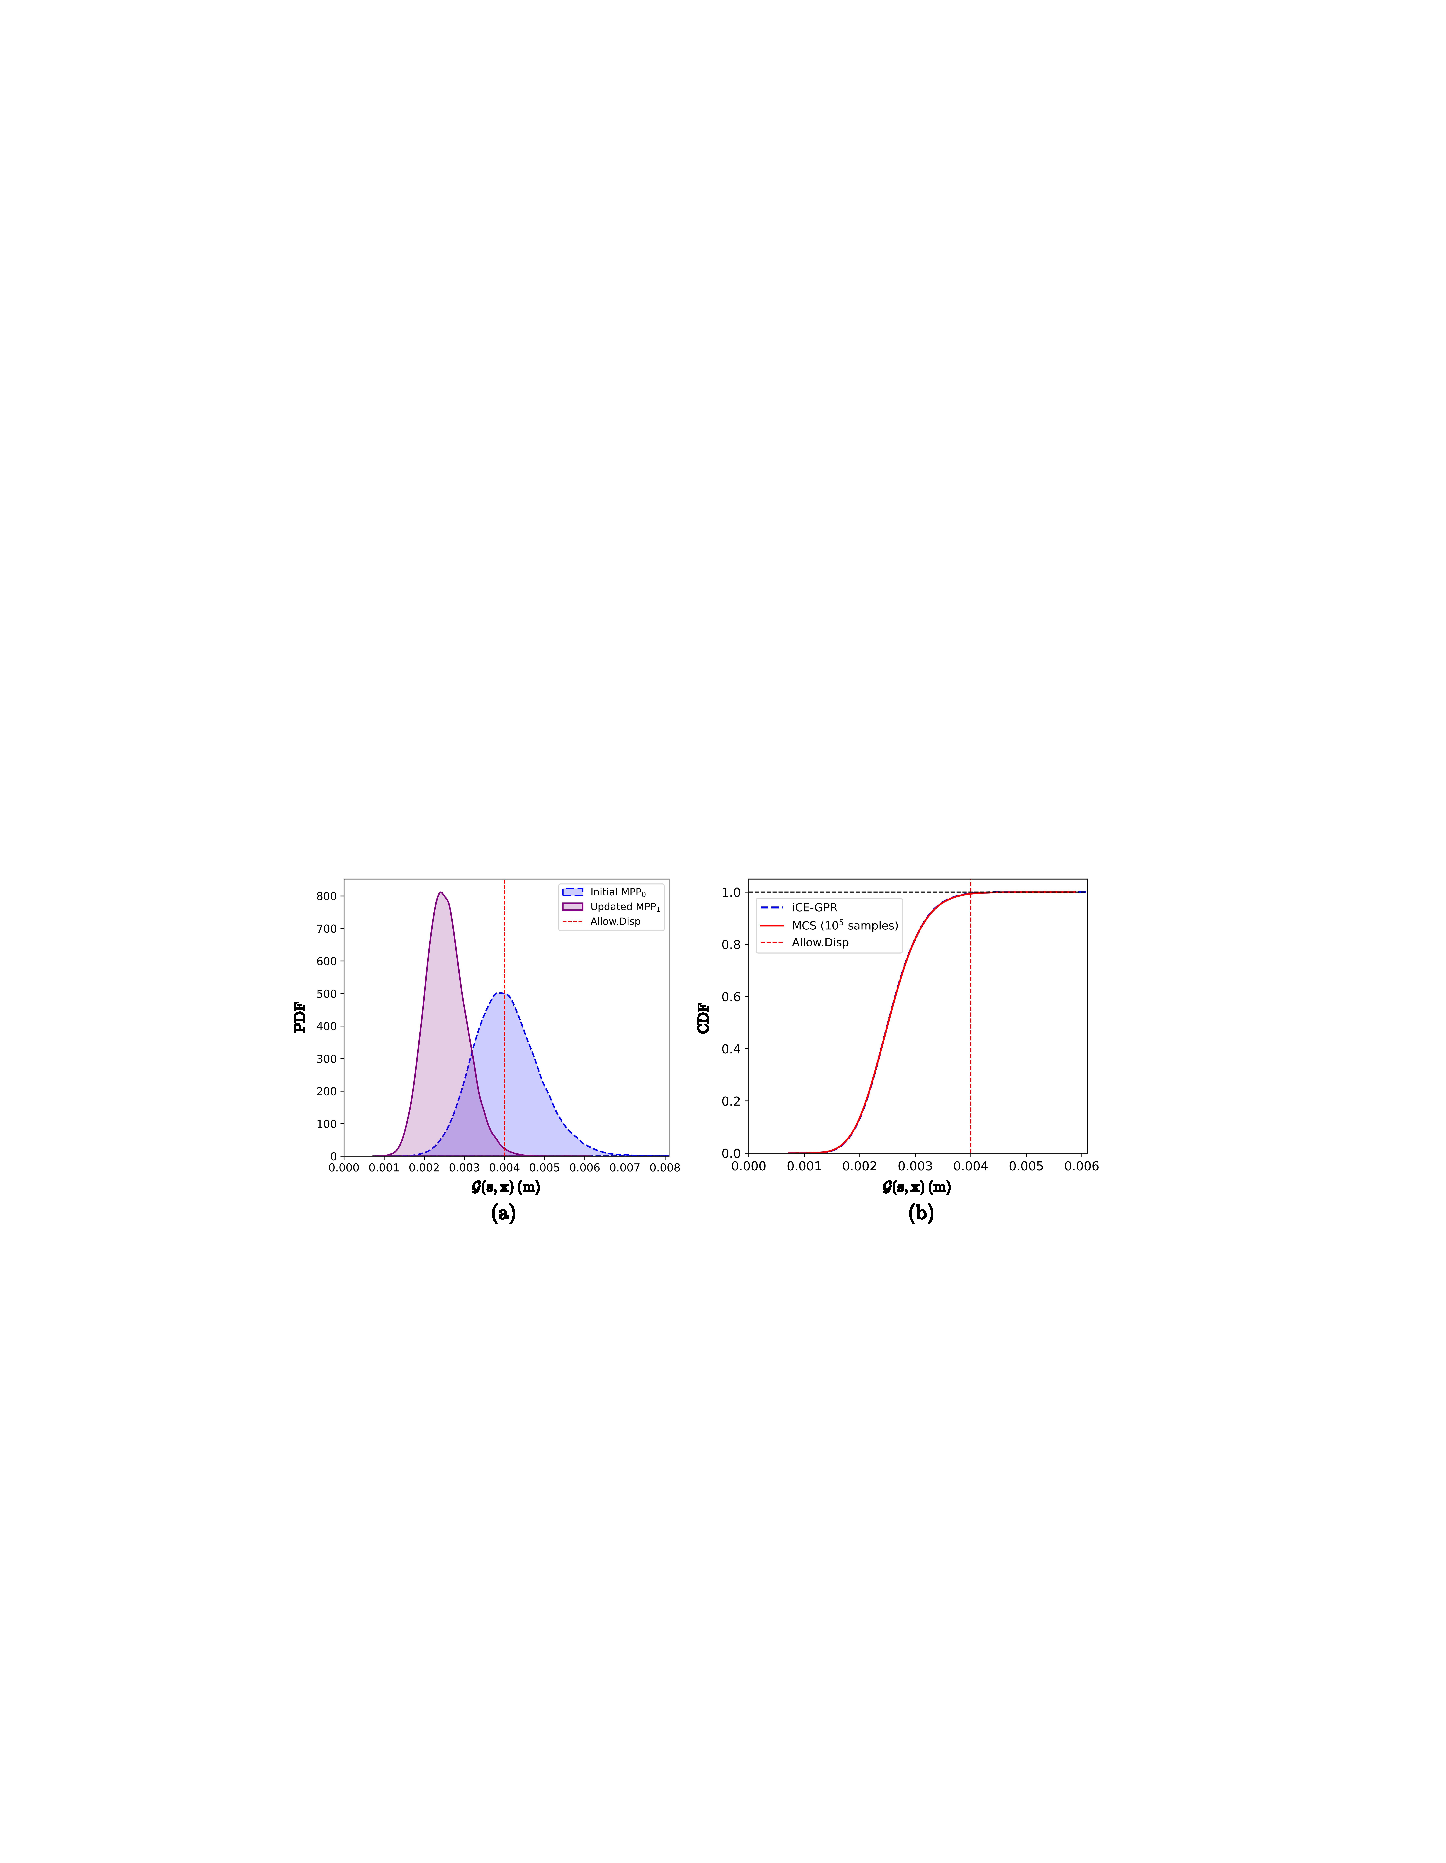
\includegraphics[scale=1.185]{Fig6.jpg}
    \end{center}
    \caption{Example 1: (a) Histories of PDFs of $\mathcal{G}(\textbf{s},\textbf{x})$ during the optimization process, (b) Comparison of CDFs of $\mathcal{G}(\textbf{s},\textbf{x})$ generated by the proposed iCE-GPR and direct MCS.}
    \label{FIG:6}
\end{figure}

\Cref{FIG:6}(a) show the PDFs of the performance function $\mathcal{G}(\textbf{s},\textbf{x})$ at the optimal designs corresponding to the MPP updates. As is clear, the PDF iteratively moved the performance function $\mathcal{G}(\textbf{s},\textbf{x})$ away from its allowable value of $4\times10^{-4}\,\text{m}$ and also reduced the failure probability associated with the MPP design during the optimization process.

To further verify the feasibility and accuracy of the obtained design in \cref{Table2}, the direct MCS reliability analysis with $10^5$ samples was performed to capture the CDF of the performance function $\mathcal{G}(\textbf{s},\textbf{x})$ at the final MPP update. \Cref{FIG:6}(b) shows that the CDFs generated by the direct MCS and those obtained from the iCE-GPR were almost identical, which demonstrates the robustness of embedding the active learning process into the proposed iCE-GPR method in terms of accurate estimation of the performance function for implementing the reliability analysis. 

\subsection{Example 2: three-bay, three-story steel frame structure}\label{SUBSEC:42}

%Figure 7
\begin{figure}[ht]
    \begin{center}
        \includegraphics[scale=0.85]{Fig7.jpg}
    \end{center}
    \caption{Example 2: (a) Three-bay three-story steel frame; (b) Bi-linear model of the steel; (c) Dimensions of three steel sections used for the frame design.}
    \label{FIG:7}
\end{figure}

% Table 3
\begin{table}[ht]
	\caption{Example~2: probabilistic properties of random parameters.}
	\label{Table3}
	\begin{center}
		\scalebox{0.85}{
			\begin{tabular}{cllccc}
				\hline \noalign{\smallskip}
				No & Variable & Description & Distribution & Mean value & COV\\
				\hline \noalign{\smallskip}
				$1$&    $E_1$ [GPa]&    Elastic modulus of section 1&   Lognormal&  $206$&  $0.10$\\
				$2$&    $E_2$ [GPa]&    Elastic modulus of section 2&   Lognormal&  $206$&  $0.10$\\
				$3$&    $E_3$ [GPa]&    Elastic modulus of section 3&   Lognormal&  $206$&  $0.10$\\
				$4$&    $F_{\text{y}1}$ [MPa]&  Yield stress of section 1&  Lognormal&  $360$&  $0.10$\\
				$5$&    $F_{\text{y}2}$ [MPa]&  Yield stress of section 2&  Lognormal&  $360$&  $0.10$\\
				$6$&    $F_{\text{y}3}$ [MPa]&  Yield stress of section 3&  Lognormal&  $360$&  $0.10$\\
				$7$&    $b_1$ [kN]& Hardening parameter of section 1&   Lognormal&  $0.02$& $0.05$\\
				$8$&    $b_2$ [kN]& Hardening parameter of section 2&   Lognormal&  $0.02$& $0.05$\\
				$9$&    $b_3$ [kN]& Hardening parameter of section 3&   Lognormal&  $0.02$& $0.05$\\
				$10$&   $P_1$ [kN]& Gravity load at external frame connections& Lognormal&  $50$&   $0.15$\\
				$11$&   $P_2$ [kN]& Gravity load at internal frame connections& Lognormal&  $100$&  $0.15$\\
				$12$&   $F$ [kN]&   Lateral load at top floor&  Lognormal&  $300$&  $0.20$\\
				\hline \noalign{\smallskip}
		\end{tabular}}
	\end{center}
\end{table}

%Figure 8
\begin{figure}[h!]
	\begin{center}
		\includegraphics[scale=0.7]{Fig8.jpg}
	\end{center}
	\caption{Example 2: convergence histories of the total area and failure probability.}
	\label{FIG:8}
\end{figure}

A three-bay three-story steel frame \cite{Xu2019} in \cref{FIG:7}(a) was investigated. The frame has 21 structural members, categorized into 3 independent groups of columns and beams ($n_\text{s}$ = 3), as shown in \cref{FIG:7}(a), with each group consisting of the identical I-section as depicted in \cref{FIG:7}(c). The depth $d$, web thickness $t_\text{w}$, flange width $b_\text{f}$, and flange thickness $t_\text{f}$ of the section for each group were the design variables. The constraints imposed the bounds on these variables, including $d \in [200, 300]$ mm, $t_\text{w} \in [16, 24]$ mm, $b_\text{f} \in [200, 300]$ mm and $t_\text{f} \in [16, 24]$ mm. The frame was designed to minimize the total cross-sectional area of the three I-sections under uncertainty in material properties, gravity loads, and lateral loads. The stress–strain relationship for the steel material of the section in each group was idealized as being uniaxial-bilinear elastoplastic, as shown in \cref{FIG:7}(b), that is characterized by three parameters: Young’s modulus $E$, the initial yield stress $F_y$, and the hardening parameter $b$ defined as the ratio of the post-yield tangent to initial elastic tangent. Thus, there were nine random material parameters for the three-member groups of the frame. The gravity loads were assigned respectively at the external and internal connections of the steel frame including $P_1$ and $P_2$ at the external and internal connections. The lateral loads applied linearly varied with the height of the frame, as shown in \cref{FIG:7}(a), with the maximum value $F$ at the top floor. Detailed probabilistic properties of the aforementioned random material parameters, gravity loads, and lateral loads are listed in \cref{Table3}. Moreover, the lateral drift of the third floor, denoted as $\Delta$, was considered as the performance of interest whose probability of exceeding an allowable value of $8\times10^{-2}\,\text{m}$ must be less than or equal to $\mathcal{P}_\text{a}$ = $1.34\times10^{-3}$. Thus, the RBDO problem of the steel frame was 
%Equation 27
\begin{equation}
    \begin{aligned}
        \underset{\textbf{s}}{\text{minimize}} \quad & \mathcal{C}(\textbf{s}) = \displaystyle\sum_{e=1}^{3} \left(d_e-2t_{\text{f}e})t_{\text{w}e}+2b_{\text{f}e}t_{\text{f}e}\right)\\
        \text{subject to} \quad &
        \mathbb{P}\bigl[\mathcal{G}(\textbf{s},\textbf{x})-8\times10^{-2} \geq 0\bigr]-\mathcal{P}_{\text{a}} \leq 0 \,; \mathcal{G}(\textbf{s},\textbf{x}) = \Delta,\\
        & s_e =\{d_e,t_{\text{w}e},b_{\text{f}e},t_{\text{f}e}\} \,; d \in \{1,\dots,3\},\\
        & d_e \in [200,300]\times10^{-3}\,\text{m}\,; t_{\text{w}e} \in [16,24]\times10^{-3}\,\text{m},\\
        & b_{\text{f}e} \in [200,300]\times10^{-3}\,\text{m}\,; t_{\text{f}e} \in [16,24]\times10^{-3}\,\text{m}.
    \end{aligned}
    \label{EQ:27}
\end{equation}

The elastic-plastic analysis for the frame was carried out using OpenSees \cite{PEERC2020}, in which the fiber model was used to simulate the monotonic elastoplastic behavior of the structure members under load control with the load increment factor of 0.01. The moment-curvature relationship of an I-section was obtained through the integration of 14 fibers along the depth of the cross-section (ten for the web plate and two for each flange). The number of section integration points was set as five for modeling the equilibrium of each structural element; see \cref{FIG:7}(a). Geometric nonlinearity was also considered in the structural analysis.

\Cref{FIG:8} shows convergence histories of the total area $\mathcal{C}(\textbf{s})$ and the failure probability  $\mathcal{P}_\text{f}$ of the steel frame during the optimization procedure of the proposed iCE-GPR method. With the efficient iCE method, the whole optimization process required only three MPP updates to successfully converge to the optimal solution.
%In each decoupling iteration, one reliability assessment was followed by a DDO to determine the failure probability of the resulting MPP design.
At the beginning of the optimization, a small objective value resulted in a large failure probability of the corresponding current optimal design. In the consequent optimization iteration, the updated MPP considerably increased the objective function, thereby leading to a large drop in the failure probability to satisfy the allowable threshold of the failure probability. The PDF responses of the performance function $\mathcal{G}(\textbf{s},\textbf{x})$ were plotted in \cref{FIG:9}(a). As explicitly, the subsequent MPP updates finely decreased the moving distance toward the optimal design, for which the corresponding failure probability complied with the targeted value.

%Figure 9
\begin{figure}[ht]
	\begin{center}
		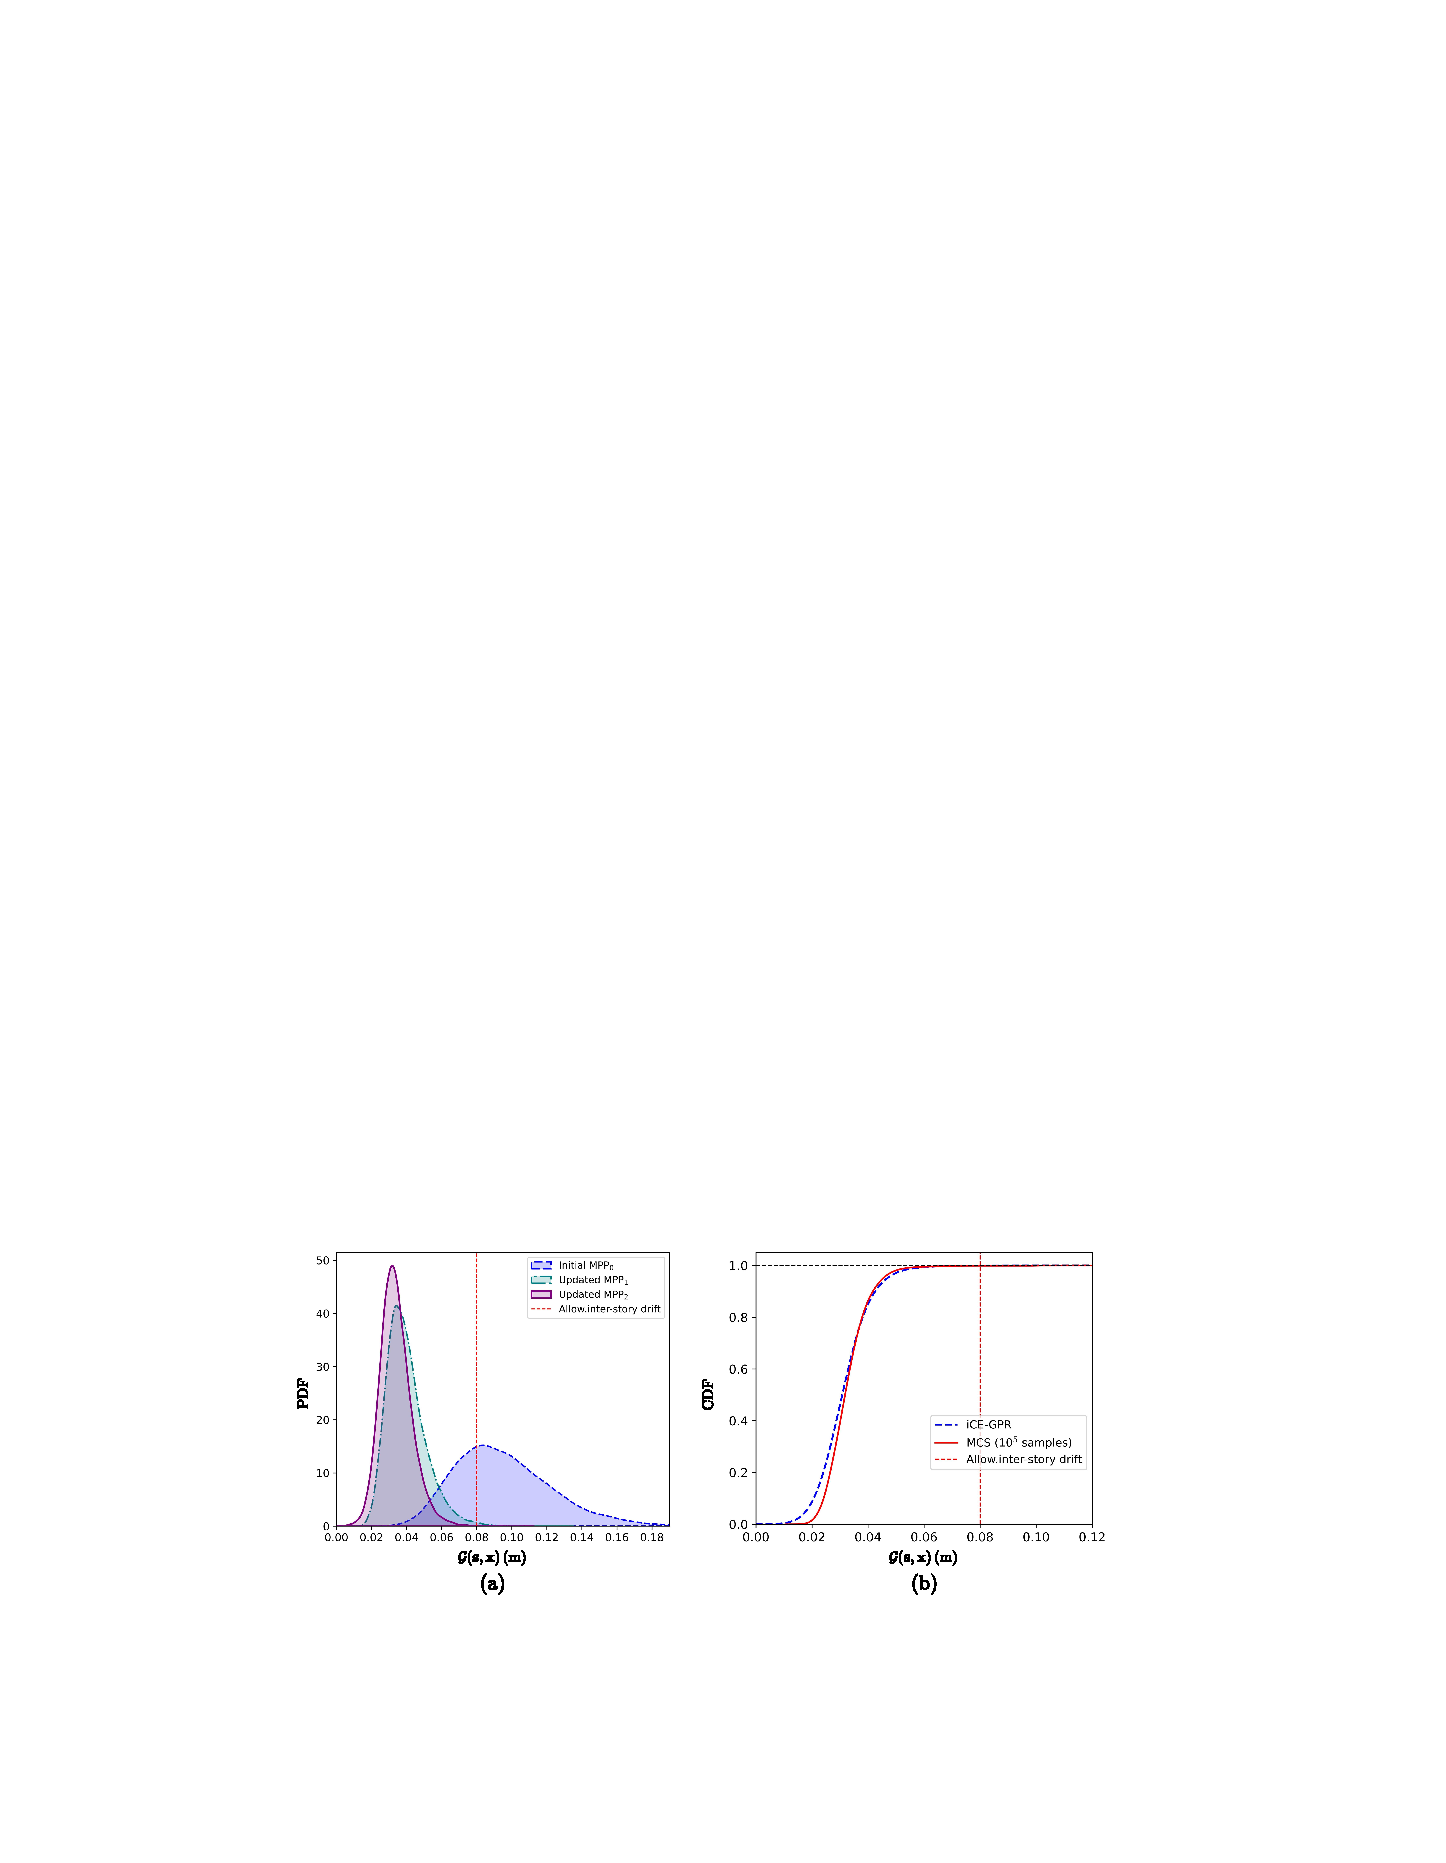
\includegraphics[scale=1.185]{Fig9.jpg}
	\end{center}
	\caption{Example 2: (a) Histories of PDFs of $\mathcal{G}(\textbf{s},\textbf{x})$ during the optimization process; (b) Comparison of CDFs of $\mathcal{G}(\textbf{s},\textbf{x})$ generated by the proposed iCE-GPR and direct MCS.}
	\label{FIG:9}
\end{figure}

%Table 4
\begin{table}[h!]
	\caption{Example~2: optimal solutions of RBDO and deterministic optimization problems.}
	\label{Table4}
	\begin{center}
		\scalebox{0.76}{
			\begin{threeparttable}
				\begin{tabular}{llccccccccc}
					\hline \noalign{\smallskip}
					Optimization attempt &  Section &   $d$&    $t_\text{w}$&   $b_\text{f}$&   $t_\text{f}$&   $\mathcal{C}(\textbf{s})$&    No. of FEAs&    CPU time&   $\mathcal{P}_\text{f}$ &  $\mathcal{P}_\text{f}$\\
					& {}& $[10^{-3}\text{m}]$& $[10^{-3}\text{m}]$& $[10^{-3}\text{m}]$& $[10^{-3}\text{m}]$& $[\text{m}^2]$& {}& [s]& (Estimated)& (MCS)\\
					\hline \noalign{\smallskip}
					\multirow{3}{*}{Deterministic CLPSO} & $s_1$ & $200.0$&  $16.0$ & $200.0$ &  $16.0$ & \multirow{3}{*}{$0.0281$} & \multirow{3}{*}{$-$} & \multirow{3}{*}{$-$} & \multirow{3}{*}{$-$} & \multirow{3}{*}{$0.4892$}\\
					& $s_2$ & $200.0$&  $16.0$& $200.0$&    $16.0$ & & & & &\\
					& $s_3$ & $253.8$&  $16.0$& $200.0$&    $16.0$ & & & & &\\
					\noalign{\smallskip}
					\multirow{3}{*}{$\text{GPR-CLPSO}$ \cite{VANHUYNH2023}} & $s_1$ & $212.1$&   $16.0$& $200.0$&    $16.0$ & \multirow{3}{*}{$0.0338$}&\multirow{3}{*}{$360 + 15^*$}&\multirow{3}{*}{ $7,216$}&\multirow{3}{*}{$0.0009$}&\multirow{3}{*}{$0.00117$}\\
					& $s_2$ & $300.0$&    $16.0$&   $211.0$&    $16.0$ & & & & &\\
					& $s_3$ & $300.0$&  $16.0$& $272.0$&    $17.0$ & & & & &\\
					\noalign{\smallskip}
					\multirow{3}{*}{$\text{Present work}$} & $s_1$ & $210.1$&   $16.0$& $200.0$&    $16.0$ & \multirow{3}{*}{$0.0337$}&\multirow{3}{*}{$360 + 15^*$}&\multirow{3}{*}{ $3,611$}&\multirow{3}{*}{$0.0012$}&\multirow{3}{*}{$0.00131$}\\
					& $s_2$ & $300.0$&    $16.0$&   $210.0$&    $16.0$ & & & & &\\
					& $s_3$ & $300.0$&  $16.0$& $271.0$&    $17.0$ & & & & &\\
					\hline \noalign{\smallskip}
				\end{tabular}
				\begin{tablenotes}
					\item * $+15$ is the total number of added points from the learning function EFF.
				\end{tablenotes}
		\end{threeparttable}}
	\end{center}
\end{table}

\cref{Table4} lists the deterministic optimal design of the steel frame associated with the mean vector of the random parameters and the optimal design obtained by the proposed iCE-GPR method. The deterministic design reported the identical solution found in the first iteration of the decoupling process, viz., the total area of $0.0281\text{m}^2$ but with an invalid failure probability of 0.4892. The total areas found by the proposed iCE-GPR was $0.0337\text{m}^2$, which is slightly lighter than those obtained from the GPR-CLPSO ($0.0344\text{m}^2$) \cite{VANHUYNH2023}, where the associated failure probability ($\mathcal{P}_\text{f}$ = $1.2\times10^{-3}$) is better than the failure probability of the GPR-CLPSO ($\mathcal{P}_\text{f}$ = $9\times10^{-4}$) \cite{VANHUYNH2023}, well-satisfied the target failure probability $\mathcal{P}_\text{a}$ = $1.34\times10^{-3}$ and is very close to the unbiased failure probability of $1.31\times10^{-3}$ reported by the corresponding direct MCS with $10^5$ random samples. The total number of FEA calls required to furnish the reliability analysis involved only 375 analyses. The CPU time recorded for the proposed iCE-GPR was 3,611 s, which is significantly less than 7,216 s for the GPR-CLPSO \cite{VANHUYNH2023}. 

To further verify the feasibility of the obtained optimal designs in \cref{Table4}, the direct MCS reliability analyses with $10^5$ random samples were performed to capture the CDF of the performance function $\mathcal{G}(\textbf{s},\textbf{x})$ associated with the final optimal design. The resulting CDFs were also compared with those obtained from the proposed iCE-GPR method. A good agreement is that the CDFs generated by the iCE-GPR and by the direct MCS over the failure domain were similar as shown in \cref{FIG:9}(b). This can be explained by the success of performing the EFF refinement in the vicinity of the response threshold.

%Figure 10
\begin{figure}[t]
	\begin{center}
		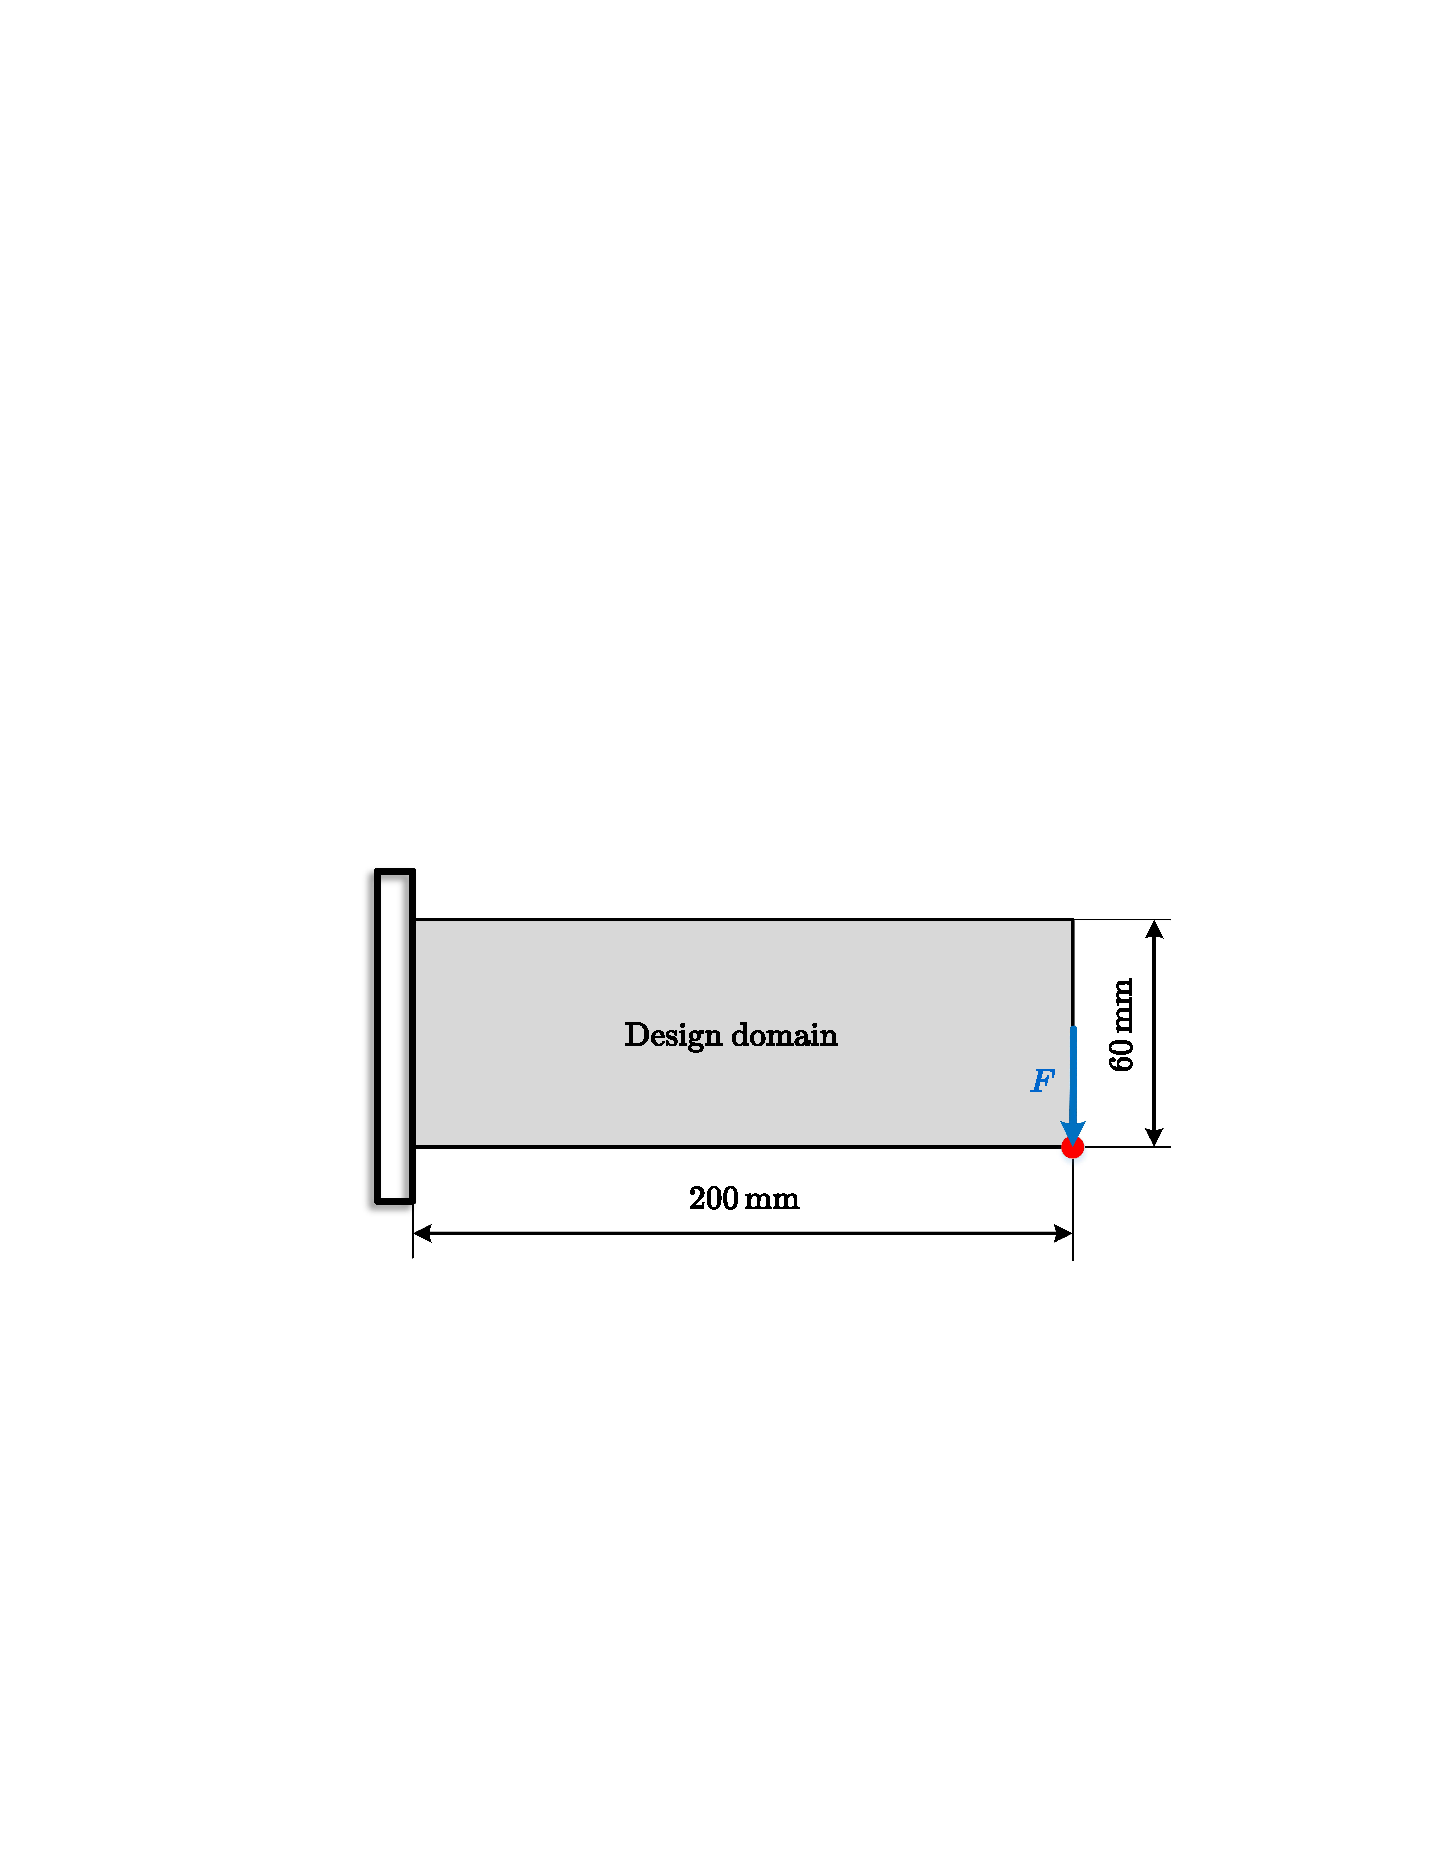
\includegraphics[scale=0.6]{Fig10.jpg}
	\end{center}
	\caption{Example 3: design domain and boundary conditions of the 2D rectangular cantilever beam.}
	\label{FIG:10}
\end{figure}

%Table 5
\begin{table}[t]
	\caption{Example~3: probabilistic properties of random parameters.}
	\label{Table5}
	\begin{center}
		\begin{tabular}{lccc}
			\hline \noalign{\smallskip}
			Variable & Distribution & Mean value & COV\\
			\hline \noalign{\smallskip}
			$E$ [GPa] &    Normal  & $1$ & $0.05$\\
			$\upsilon$ &    Normal &    $0.3$ &  $0.05$\\
			$F$ [N] &    Normal &    $100$ &  $0.05$\\
			\hline \noalign{\smallskip}
		\end{tabular}
	\end{center}
\end{table}

%Table 6
\begin{table}[t!]
	\caption{Example~3: optimization results from DTO and RBTO problems.}
	\label{Table6}
	\begin{center}
		\scalebox{0.9}{
			\begin{threeparttable}
				\begin{tabular}{llccccccccc}
					\hline \noalign{\smallskip}
					Optimization attempt & $\mathcal{C}(\textbf{s})$&    No. of FEAs&    CPU time&   $\mathcal{P}_\text{f}$ &  $\mathcal{P}_\text{f}$\\
					& $[\%]$& {}& [s]& (Estimated)& (Direct MCS)\\
					\hline \noalign{\smallskip}
					$\text{DTO}$&    $47.24$&    $-$&   $-$&  $-$&  $0.49996$\\
					%\hline
					$\text{iCE-GPR}$&    $62.89$&    $60+10$&   $428$&  $0.00131$&  $0.00124$\\
					\hline \noalign{\smallskip}
				\end{tabular}
				\begin{tablenotes}
					\item * $+10$ is the total number of added points from the learning function EFF.
				\end{tablenotes}
		\end{threeparttable}}
	\end{center}
\end{table} 

\subsection{Example 3: 2D rectangular cantilever beam}\label{SUBSEC:43}
The third example considered the volume minimization of a 2D rectangular cantilever beam under plane stress assumption, as drawn in \cref{FIG:10}. The design domain was discretized into $n_\text{e}$ = 12,000 (200 mm $\times$ 60 mm) quadrilateral finite elements, while the left edge of the cantilever beam was fixed and a concentrated force $F$ was exerted vertically at the bottom point of the right edge. The material properties included Young’s modulus $E_0$ and the poison’s ratio $\upsilon$. $F$, $E_0$, and $\upsilon$ were considered the random parameters $\textbf{x}$ as detailed in \cref{Table5}. The maximum vertical displacement, denoted as $\Delta$, was considered as the performance of interest, whose probability of exceeding an allowable displacement of 25 mm must be less than or equal to $\mathcal{P}_\text{a}$ = $1.34\times10^{-3}$. Thus, the RBTO problem of this example was formulated as follows:
%Equation 28
\begin{equation}
    \begin{aligned}
        \underset{\textbf{s}}{\text{minimize}} \quad & \mathcal{C}(\textbf{s}) = \displaystyle\sum_{e=1}^{n_\text{e}} s_e\\
        \text{subject to} \quad &
        {\bf K(s)}{\bf u}={\bf F},\\
        & \mathbb{P}\bigl[\mathcal{G}(\textbf{s},\textbf{x})-25 \geq 0 \bigr]-\mathcal{P}_{\text{a}} \leq 0 \,; \mathcal{G}(\textbf{s},\textbf{x}) = \Delta,\\
        &s_e \in [0.001,1]; e \in \{1,\dots,n_\text{e}\}.
    \end{aligned}
    \label{EQ:28}
\end{equation}

%Figure 11
\begin{figure}[t]
	\begin{center}
		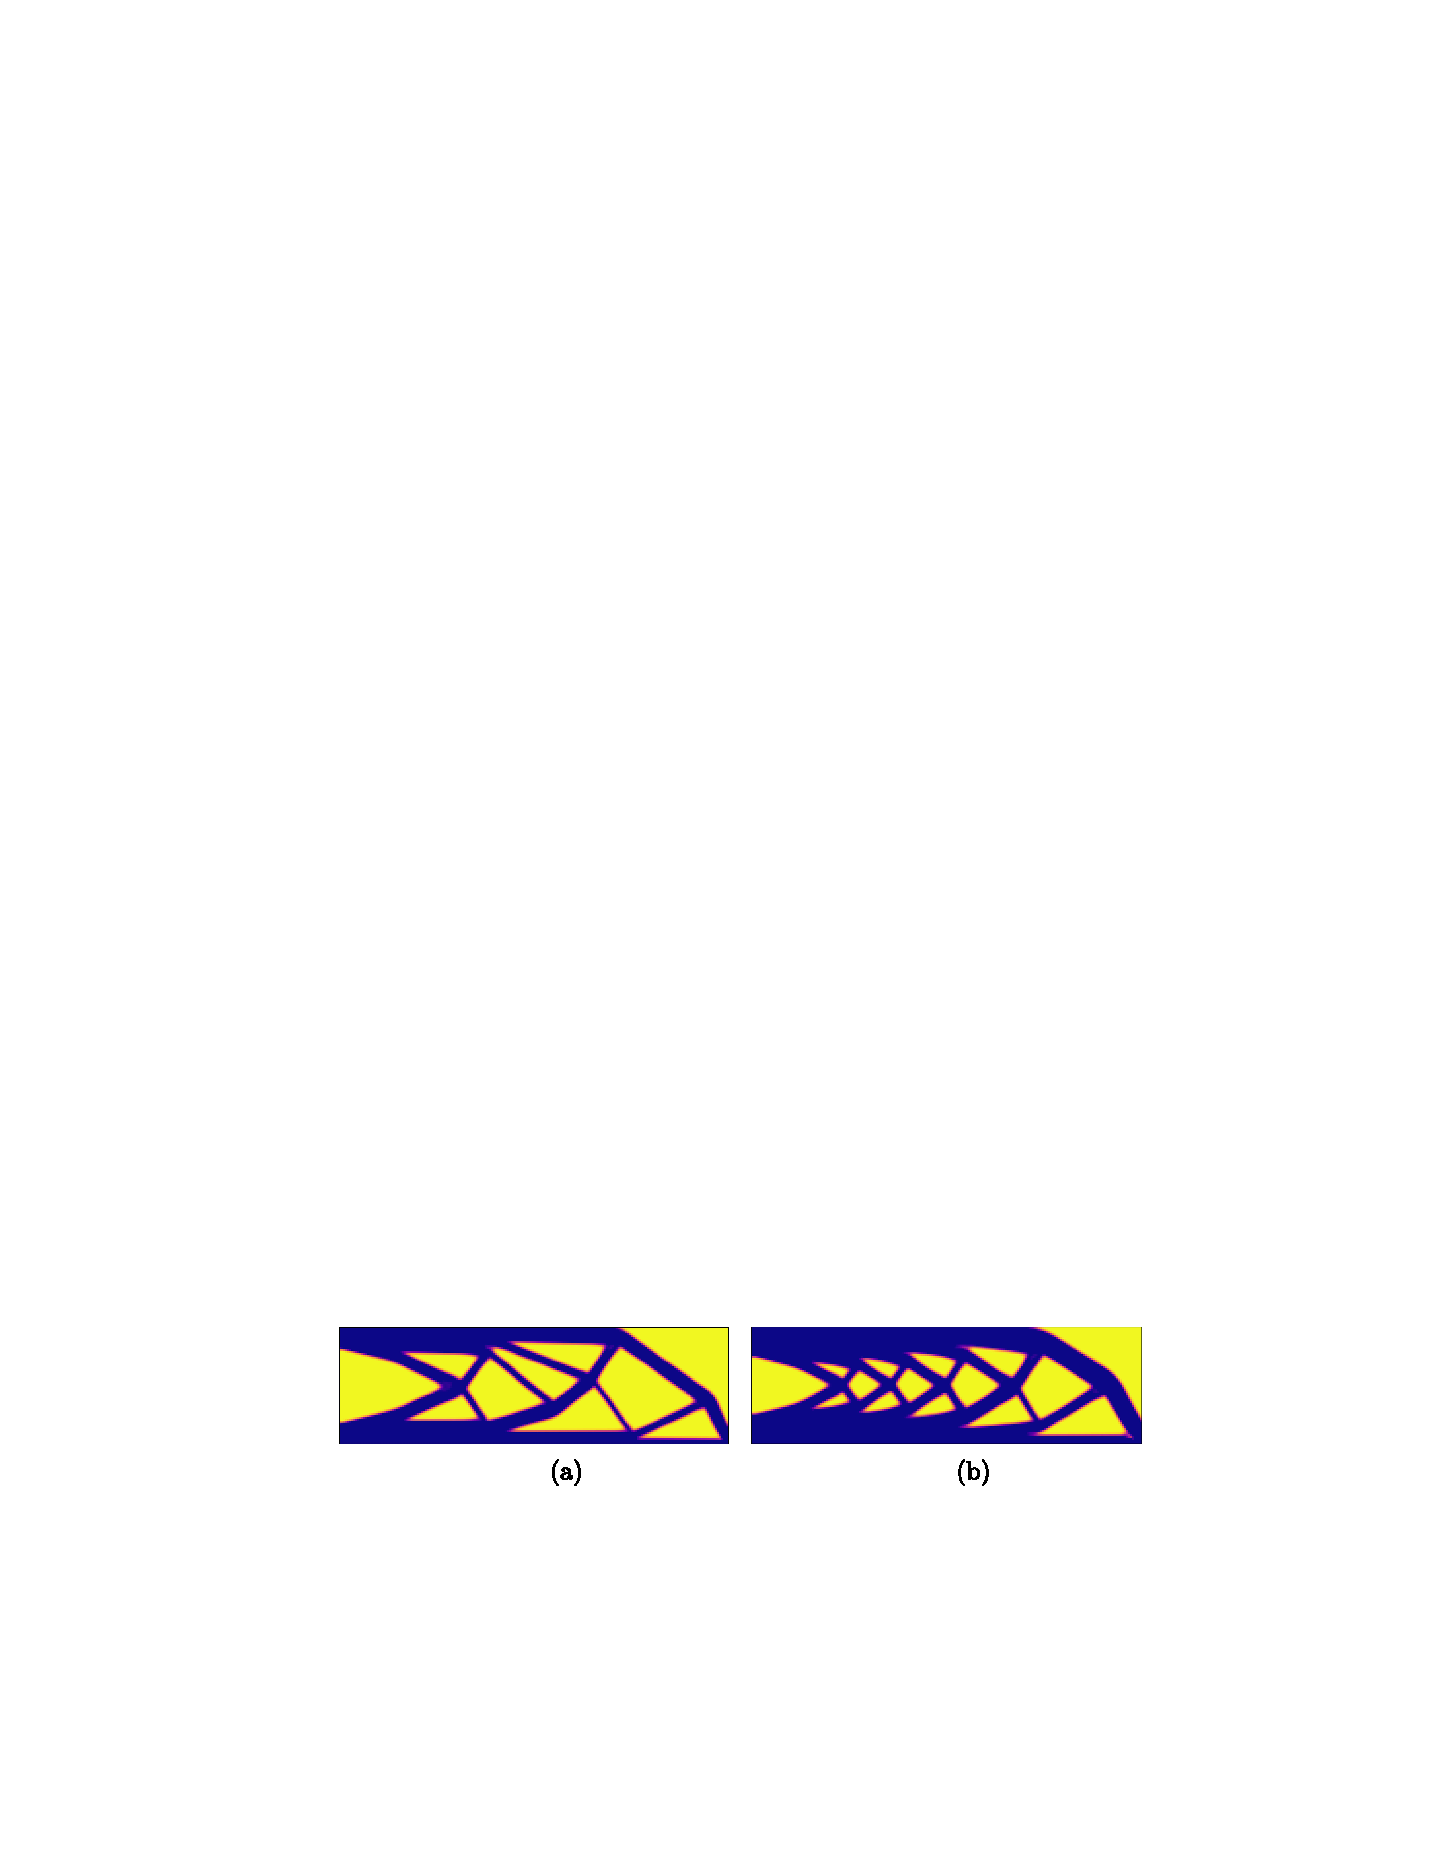
\includegraphics[scale=1.2]{Fig11.jpg}
	\end{center}
	\caption{Example 3: optimal topology solutions from (a) the DTO problem and (b) the RBTO problem.}
	\label{FIG:11}
\end{figure}

\cref{Table6} and \cref{FIG:11} provide the optimization results found by the deterministic topology optimization (DTO) and the proposed iCE-GPR method. The DTO offered the smallest optimal volume of 47.24\% and an unacceptable failure probability of 0.49996.
While the proposed iCE-GPR provided the optimal volume of 62.89\%, the associated failure probability was $1.31\times10^{-3}$, which well satisfies the threshold value of $\mathcal{P}_\text{a}$ =  $1.34\times10^{-3}$ and fully agrees with the true failure probability of $1.24\times10^{-3}$ from the direct MCS with $10^5$ random samples. In terms of computational efficiency, the proposed iCE-GPR took only 70 FEA runs to complete reliability analysis in correspondence to the optimal topology structure. The CPU time for the whole RBTO procedure was only 428 s. 
\Cref{FIG:12}(a) illustrates the evolution of the PDF of the $\mathcal{G}(\textbf{s},\textbf{x})$ during the optimization process. With the efficiency of the iCE method, the whole RBTO process required only two MPP updates. %This evidenced that the proposed iCE-GPR method quickly captured the optimal design solution. As observed in \cref{FIG:12}(a), the PDFs quickly moved the performance function $\mathcal{G}(\textbf{s},\textbf{x})$ away from its allowable displacement value of 25 mm, thereby step-by-step reducing the failure probability associated with the MPP update during the decoupling RBTO process. 

The direct MCS with $10^5$ random samples was performed to capture the CDF of the performance function $\mathcal{G}(\textbf{s},\textbf{x})$ corresponding to the optimal topology solution. \Cref{FIG:12}(b) shows that the CDFs drawn by the direct MCS method and the iCE-GPR method are similar. The robustness of the iCE-GPR method integrating with the EFF refinement was thus evidenced.
%The proposed method accurately furnished the reliability analyses and performance function under the decoupling RBTO procedures.

%Figure 12
\begin{figure}
	\begin{center}
		\includegraphics[scale=1.2]{Fig12.jpg}
	\end{center}
	\caption{Example 3: (a) Histories of PDFs of $\mathcal{G}(\textbf{s},\textbf{x})$ during the optimization process; (b) Comparison of CDFs of $\mathcal{G}(\textbf{s},\textbf{x})$ generated by the proposed iCE-GPR and direct MCS.}
	\label{FIG:12}
\end{figure}

\subsection{Example 4: 3D cantilever-beam structure}\label{SUBSEC:44}
The last example optimized the volume of a 3D cantilever-beam structure subjected to a sine-shaped load at the bottom of the free edge. The sine function has a value of zero at the two corners and $q_\text{mid}$ at the midpoint. The loading, boundary condition, and design domain are shown in \cref{FIG:13}. The finite element mesh consists of $48 \times 24 \times 24$ unity cubes, or equivalently the number of elements is $n_\text{e}$ = 27,648. This example was considered a large-scale reliability problem with the need for expensive computational efforts in the FEA. The material properties were $E_0$, and the poison’s ratio $\upsilon$. The distributions of $q_\text{mid}$, $E_0$, and $\upsilon$ are listed in \cref{Table7}. The maximum compliance denoted $\mathfrak{C}$, was considered as the performance of interest, whose probability of exceeding allowable compliance of 3,330 N/mm must be less than or equal to $\mathcal{P}_\text{a}$ = $1.34\times10^{-3}$. Thus, the governing RBTO problem of this example was formulated as
%Equation 29
\begin{equation}
    \begin{aligned}
        \underset{\textbf{s}}{\text{minimize}} \quad & \mathcal{C}(\textbf{s}) = \displaystyle\sum_{e=1}^{n_\text{e}} s_e\\
        \text{subject to} \quad &
        {\bf K(s)}{\bf u}={\bf F},\\
        &\mathbb{P}\bigl[\mathcal{G}(\textbf{s},\textbf{x})-3,330 \geq 0 \bigr]-\mathcal{P}_{\text{a}} \leq 0 \,; \mathcal{G}(\textbf{s},\textbf{x}) = \mathfrak{C},\\
        &s_e \in [0.001,1]; e \in \{1,\dots,n_\text{e}\}.
    \end{aligned}
    \label{EQ:29}
\end{equation}

%Figure 13
\begin{figure}
	\begin{center}
		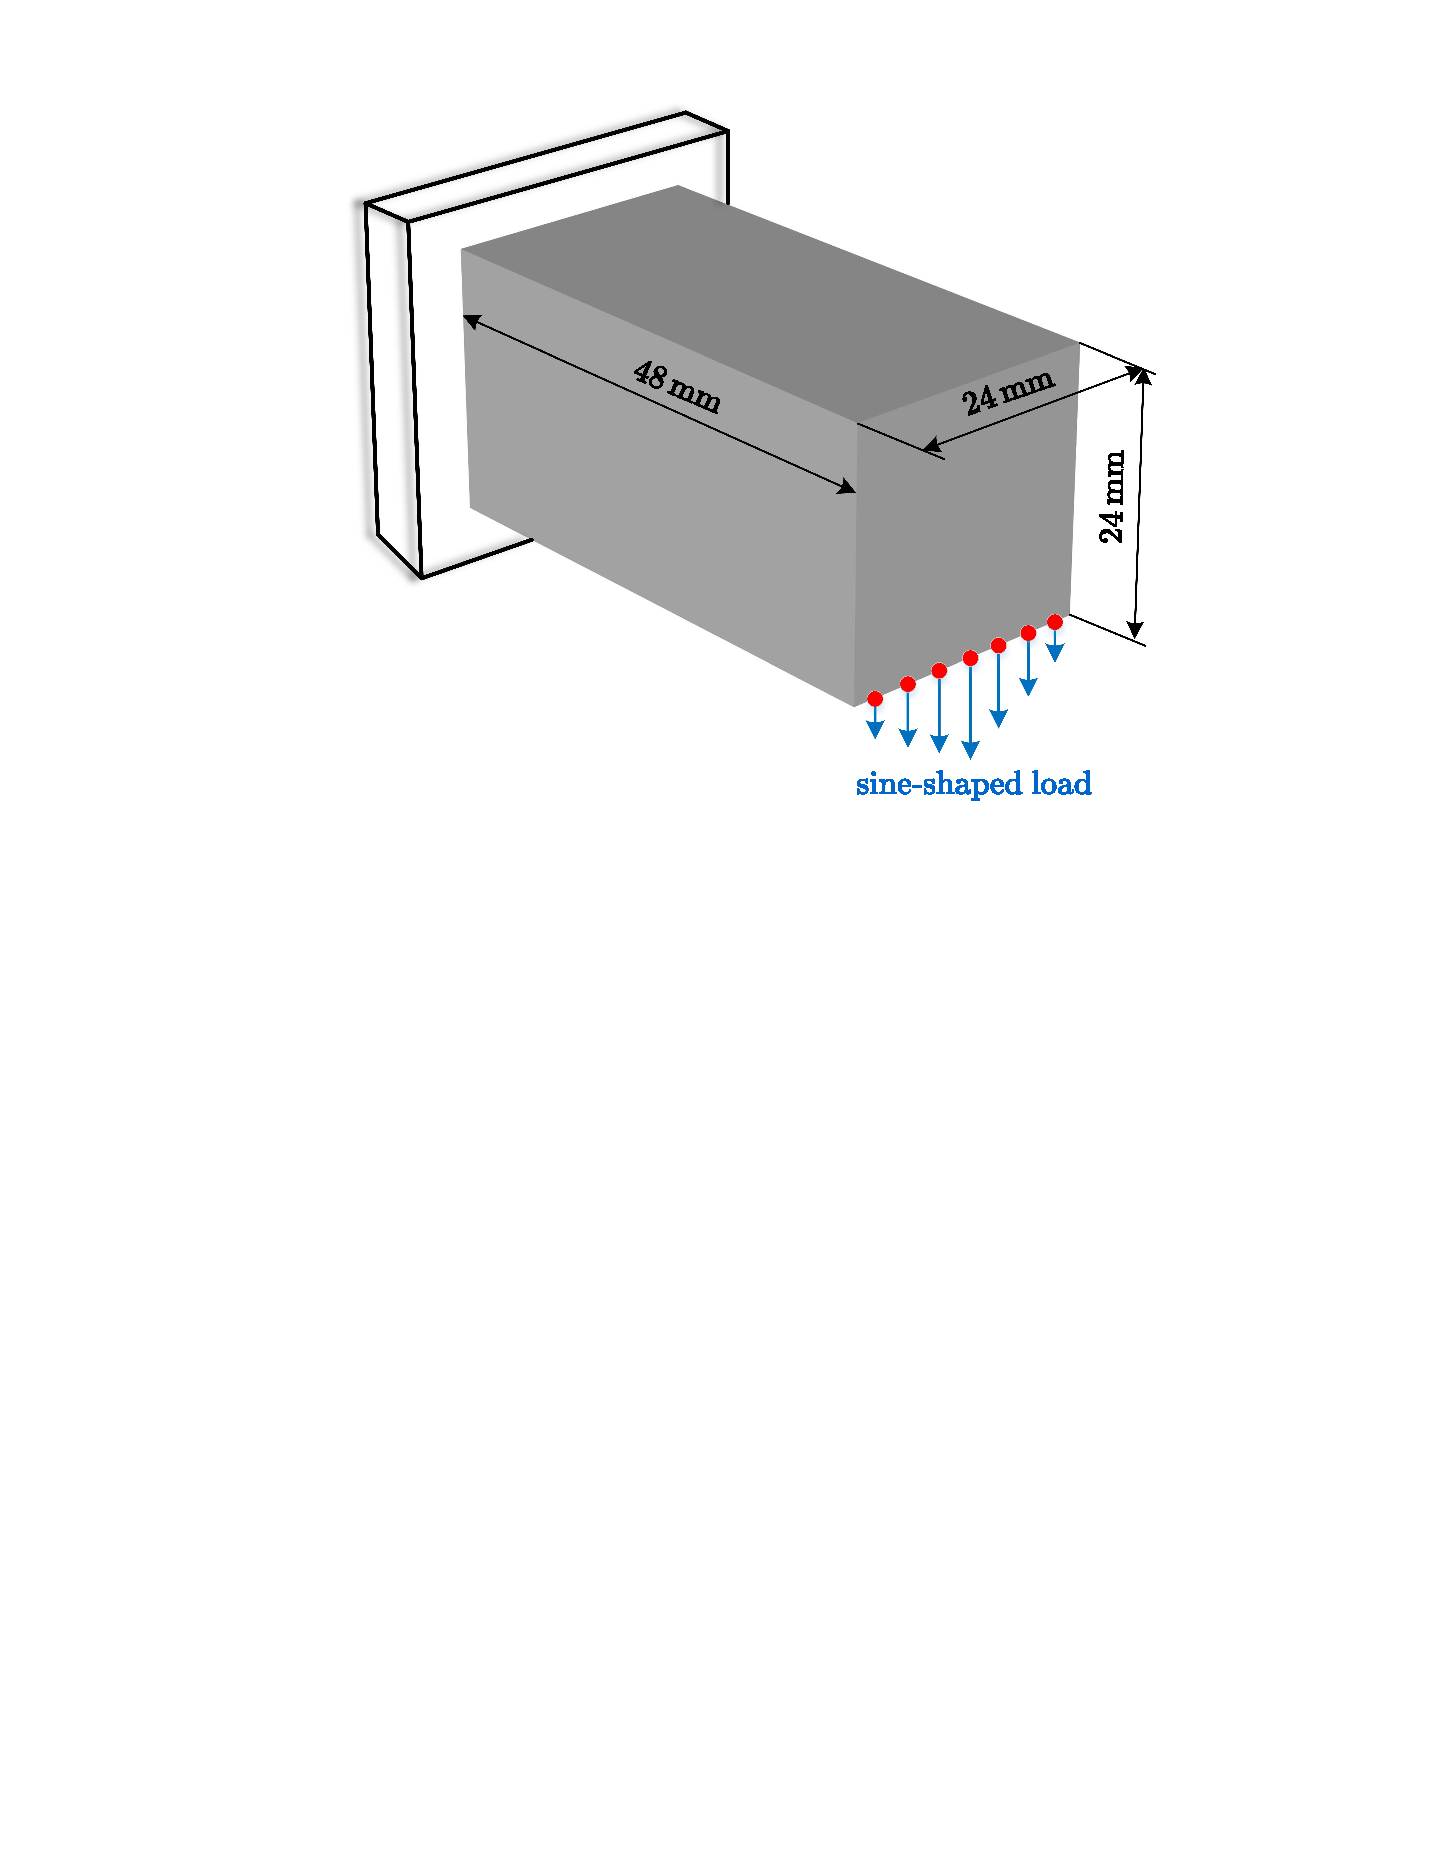
\includegraphics[scale=0.58]{Fig13.jpg}
	\end{center}
	\caption{Example 4: design domain and boundary conditions of the 3D cantilever-beam structure.}
	\label{FIG:13}
\end{figure}

%Table 7
\begin{table}
    \caption{Example~4: probabilistic properties of random parameters.}
    \label{Table7}
    \begin{center}
        \begin{tabular}{lccc}
            \hline \noalign{\smallskip}
            Variable & Distribution & Mean value & COV\\
            \hline \noalign{\smallskip}
            $E$ [MPa] &    Normal  & $1$ & $0.05$\\
            $\upsilon$ &    Normal &    $0.3$ &  $0.05$\\
            $q_\text{mid}$ [N] &    Normal &    $1$ &  $0.05$\\
            \hline \noalign{\smallskip}
        \end{tabular}
    \end{center}
\end{table}

%Figure 14
\begin{figure}[t]
	\begin{center}
		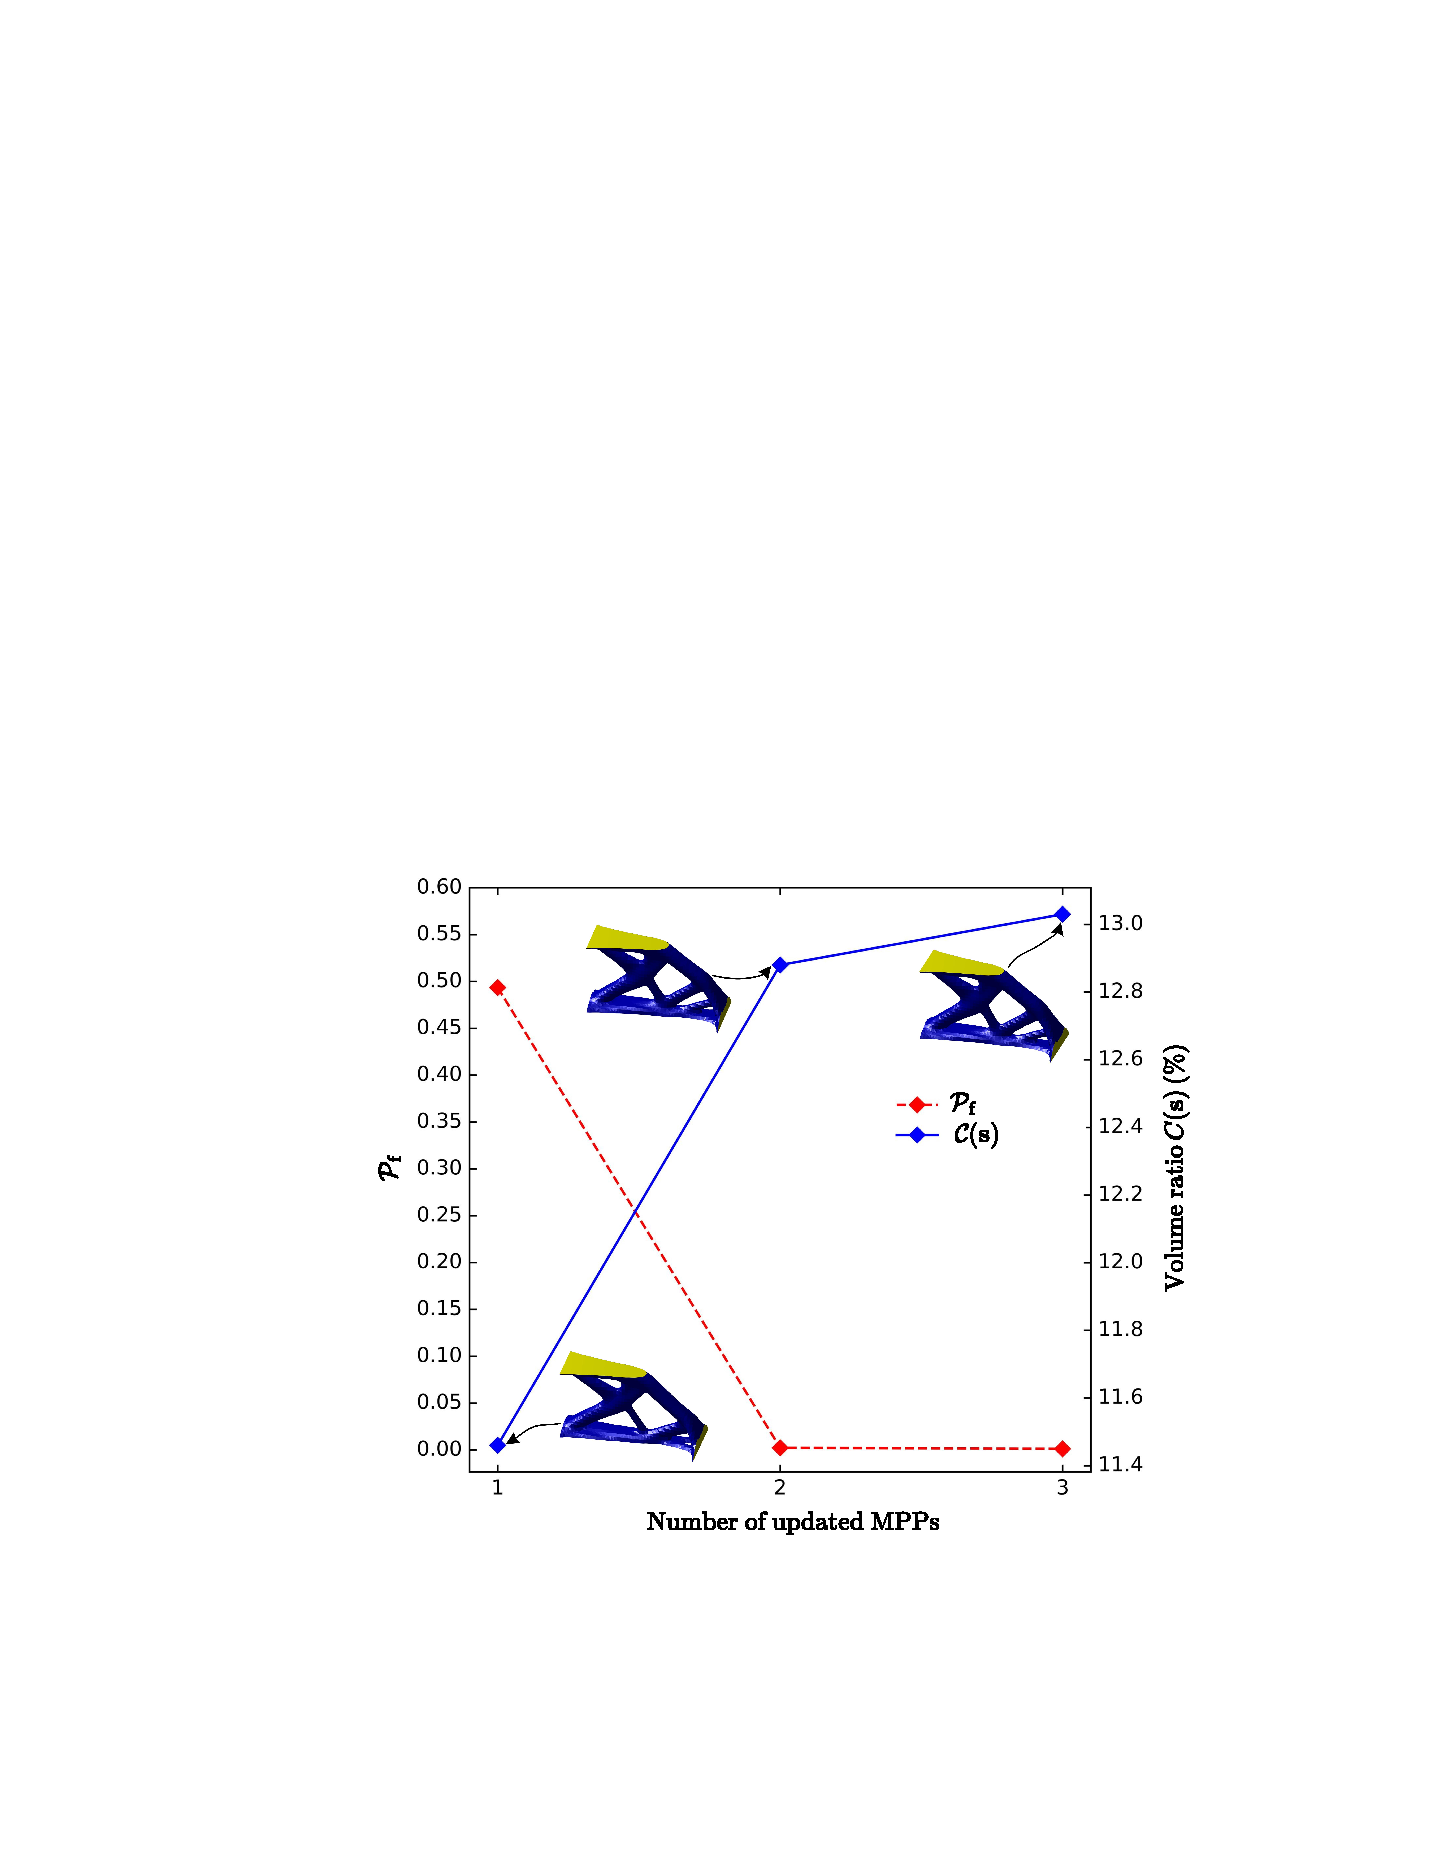
\includegraphics[scale=0.7]{Fig14.jpg}
	\end{center}
	\caption{Example 4: convergence histories of the total volume and failure probability.}
	\label{FIG:14}
\end{figure}

%Table 8
\begin{table}[t]
	\caption{Example~4: optimization results of the DTO and RBTO problems.}
	\label{Table8}
	\begin{center}
		\scalebox{0.9}{
			\begin{threeparttable}
				\begin{tabular}{llccccccccc}
					\hline \noalign{\smallskip}
					Optimization attempt & $\mathcal{C}(\textbf{s})$&    No. of FEAs&    CPU time&   $\mathcal{P}_\text{f}$ &  $\mathcal{P}_\text{f}$\\
					& $[\%]$& {}& [s]& (Estimated)& (Direct MCS)\\
					\hline \noalign{\smallskip}
					$\text{DTO}$&    $11.46$&    $-$&   $-$&  $-$&  $0.49345$\\
					%\hline
					$\text{iCE-GPR}$&    $13.03$&    $90+15$&   $1,829$&  $0.00119$&  $0.00121$\\
					\hline \noalign{\smallskip}
				\end{tabular}
				\begin{tablenotes}
					\item * $+15$ is the total number of added points from the learning function EFF.
				\end{tablenotes}
		\end{threeparttable}}
	\end{center}
\end{table}

\Cref{FIG:14} shows convergence histories of the total volume $\mathcal{C}(\textbf{s})$ and the failure probability $\mathcal{P}_\text{f}$ for the 3D cantilever-beam structure given by the proposed iCE-GPR. Like its excellent performance demonstrated in the first three examples, the proposed method quickly offered the optimal topology solution as the whole RBTO process performed only three MPP updates. The evolution of the PDF of the $\mathcal{G}(\textbf{s},\textbf{x})$ during the optimization process was plotted in \cref{FIG:16}(a). In each optimization iteration, the first MPP update quickly identified and moved the PDF of $\mathcal{G}(\textbf{s},\textbf{x})$ toward the safe region with the design variable $\textbf{s}$ updates. The failure probability of the design in the final iteration achieved the target value, and then the decoupling RBTO terminated.

\cref{Table8} summarizes the optimal design of the deterministic 3D cantilever beam associated with the mean vector of the random parameters as well as those of the RBTO obtained by the proposed iCE-GPR method. The deterministic optimal design, as shown in \cref{FIG:15}(a), provided the smallest volume of 11.46\% but with an invalid failure probability of 0.49345. The proposed iCE-GPR offered 13.03\% of the initial design domain and the associated failure probability was $1.19\times10^{-3}$, which is less than the threshold value of $\mathcal{P}_\text{a}$ = $1.34\times10^{-3}$ and is very close to the true failure probability of $1.21\times10^{-3}$ obtained by the direct MCS with $10^5$ random samples at the final optimal topology design. The total number of FEA calls required to furnish the reliability analyses involved only 105 and the CPU time for the whole RBTO procedure was 1,829 s. As shown in \cref{FIG:15}(b), the RBTO procedure under the proposed iCE-GPR provided a reasonable layout of topology designs while satisfying the target failure probability. 

%Figure 15
\begin{figure}[t]
	\begin{center}
		\includegraphics[scale=0.6]{Fig15.jpg}
	\end{center}
	\caption{Example 4: optimal topology solutions from (a) the DTO problem and (b) the RBTO problem.}
	\label{FIG:15}
\end{figure}

%Figure 16
\begin{figure}[t!]
	\begin{center}
		\includegraphics[scale=1.185]{Fig16.jpg}
	\end{center}
	\caption{Example 4: (a) Histories of PDFs of $\mathcal{G}(\textbf{s},\textbf{x})$ during the optimization process; (b) Comparison of CDFs of $\mathcal{G}(\textbf{s},\textbf{x})$ generated by the proposed iCE-GPR and direct MCS.}
	\label{FIG:16}
\end{figure}

To further verify the accuracy of the obtained results in \cref{Table8}, the reliability analysis was performed using the direct MCS with $10^5$ random samples to capture the CDF of the $\mathcal{G}(\textbf{s},\textbf{x})$ at the final optimal topology solution. As observed in \cref{FIG:16}(b), the CDF responses provided by the direct MCS and the proposed iCE-GPR methods over the failure domain agreed well and thus indicated the success in performing the active learning process over the vicinity of the response threshold. 

\section{Concluding remarks}
\label{sec5}
This paper proposes the efficient iCE-GPR method that couples the iCE method with the surrogate-assisted GPR model for solving both the decoupling RBDO and RBTO problems. Starting with the DDO obtained by the CLPSO algorithm for the RBDO or the SIMP for the RBTO, the proposed method iterates through estimating the failure probability, finding a new MPP of the LSF, and updating the optimal design with the new MPP point. For handling the reliability analysis, the GPR model is constructed to replace the actual performance function using a small number of training samples of the random parameters. Based on its predictive mean and covariance functions, the GPR enables a cost-effective CE method to estimate the failure probability, and new learning points at the vicinity (highly-reliable sensitive region) of the LSFs are strategically generated through the maximization of an active learning function EFF to refine the accuracy of the failure probability in each deterministic optimization. The CLPSO algorithm was primarily employed in the optimization process, in learning the GPR hyperparameters, and in maximizing the EFF. For each reliability analysis of the optimization process, the iCE method is developed that specifies a new MPP to find a new optimal design in the next decoupling iteration. The iCE method can efficiently leverage the decoupling approach to quickly explore the region that is deemed to contain the optimal solution. As a result, the iCE method significantly reduces the total computational costs required during the decoupling process, and hence fast converges the optimal solutions. This process is carried out sequentially until the failure probability reaches the target value. The effectiveness of the proposed iCE-GPR method is well-demonstrated through four numerical examples incorporating inelastic material and/or nonlinear geometry, and continuum topology optimization with huge computing efforts, which have been successfully solved for both the decoupling RBDO and RBTO schemes. The optimization results indicate that the proposed iCE-GPR method advantageously by-passes the use of computationally expensive FEA calls in assessing the failure probability functions. For future research directions, the proposed RBDO method can be extended to practical large-scale nonlinear structural systems or dynamic systems with either multiple failure modes or higher dimensions.

% Acknowledgments
\section*{Acknowledgments}
This research has been supported under Thailand Science research and Innovation Fund Chulalongkorn University
(IND66210025). The financial support provided by Chulalongkorn University under Ratchadaphiseksomphot Endowment
Fund and Second Century Fund is acknowledged

% Appendix
\section*{Appendix: Gaussian process regression}
\label{APPE}
\setcounter{equation}{0}
\renewcommand{\theequation}{A.\arabic{equation}}
Consider a training dataset $\mathcal{D}=\left(
{\bf X},{\bf y}\right) = \{{\bf x}_i,y_i\}_{i=1}^N$ of $N$ observations, where ${\bf x}_i\in\mathbb{R}^{n_\text{x}}$ is an observation of the $n_\text{x}$-dimensional input variable vector and $y_i\in\mathbb{R}$ is the corresponding value of the output variable. 
The goal of GPR is to establish an input-output relationship using the mapping $y({\bf x}) = f({\bf x})+\tau:\mathbb{R}^{n_\text{x}} \mapsto \mathbb{R}$, where 
$f({\bf x})$ is a regression function and $\tau
\sim\mathcal{N}(0,\sigma_\text{n}^2)$ is an additive Gaussian noise with zero mean and variance $\sigma_\text{n}^2$.
This noise is assumed to be independent and identically distributed given ${\bf x}$.

GPR is a stochastic process that extends the (finite) multivariate Gaussian to model functions on infinite domains. GPR imposes a prior knowledge that any set of a finite number of output variable values has a joint multivariate Gaussian distribution. Such a distribution is characterized by a mean function $m({\bf x}) = \mathbb{E}[f({\bf x})]$ representing the central tendency of the regression function and a covariance function $\kappa({\bf x}, {\bf x}') = \mathbb{E}\big[\big(f({\bf x}) - m({\bf x})\big)\big(f({\bf x}') - m({\bf x}')\big)\big] = \text{cov}[f({\bf x}),f({\bf x}')]$ measuring the cross-covariance between the function values, such that
% Equation A.1
\begin{equation}
	f({\bf x}) \sim \mathcal{GP}\left(m({\bf x}),\kappa({ \bf x}, {\bf x}')\right).
	\label{EQ:A1}
\end{equation}

This work uses the automatic relevance determination (ARD) covariance function with separate length-scale parameters $l_d$ for each of the $n_\text{x}$ input dimensions, as~\cite{Murphy2012}:
% Equation A.2
\begin{equation}
	\kappa({\bf x},{\bf x}') = \sigma_\text{f}^2\exp\left(-\frac{1}{2}\displaystyle\sum_{j=1}^{n_\text{x}}\frac{(x_j-x_j')^2}{l_j^2}\right),
	\label{EQ:A2}
\end{equation}
where $\sigma_\text{f}$ is the output scale determining the overall variability. Thus, the hyperparameter vector characterizing GPR is $\boldsymbol{\theta} = [\sigma_\text{n},\sigma_\text{f},l_1,\dots,l_{n_\text{x}}]^T$.

The prior mean function is often set as $m({\bf x})=0$ when there is a lack of strong prior knowledge about the function tendency. Accordingly, the values of the regression function at the observations of ${\bf x}$ are distributed according to
% Equation A.3
\begin{equation}
	p({\bf f}|{\bf X})\sim\mathcal{N}\left({\bf 0},{\bf K}({\bf X},{\bf X})\right),
	\label{EQ:A3}
\end{equation}
where ${\bf f} = [f({\bf x}_i),\dots,f({\bf x}_N)]^T$, and ${\bf K}({\bf X},{\bf X})\in\mathbb{R}^{N\times N}$ is the symmetric and positive semi-definite covariance matrix of all inputs. ${\bf K}({\bf X},{\bf X})$ reads
% Equation A.4
\begin{equation}
	{\bf K}({\bf X},{\bf X}) =
	\begin{bmatrix}
		\kappa({\bf x}_1,{\bf x}_1) & \cdots & \kappa({\bf x}_1,{\bf x}_N)\\
		\vdots & \ddots & \vdots\\
		\kappa({\bf x}_N,{\bf x}_1) &\cdots & \kappa({\bf x}_N,{\bf x}_N)\\
	\end{bmatrix}.
    \label{EQ:A4}
\end{equation}

Since the additive noise is independent and identically distributed, the distribution of observations ${\bf y}$ (i.e., marginal likelihood) is also a Gaussian, which reads   
% Equation A.5
\begin{equation}
	p({\bf y}|{\bf X})\sim\mathcal{N}\left({\bf 0},{\bf C}({\bf X},{\bf X})\right),
	\label{EQ:A5}
\end{equation}
where ${\bf C}({\bf X},{\bf X}) = {\bf K}({\bf X},{\bf X}) + \sigma_\text{n}^2{\bf I}_N$ with the identity matrix ${\bf I}_N\in\mathbb{R}^{N\times N}$.

Determining the hyperparameters $\boldsymbol{\theta}$ that well explain $\mathcal{D}$ is a crucial task in constructing the GPR model.
The optimal $\boldsymbol{\theta}$, denoted as $\hat{\boldsymbol{\theta}}$, reads the maximizer of the marginal likelihood of hyperparameters $\mathcal{J}(\theta)=p({\bf y}|{\bf X},\theta)$~\cite{Schulz2018,Rasmussen2006}. Accordingly,
% Equation A.6
\begin{equation}
		\hat{\boldsymbol{\theta}}=\underset{\boldsymbol{\theta}}{\mathrm{argmax}}\,\mathcal{J}(\boldsymbol{\theta})=\underset{\boldsymbol{\theta}}{\mathrm{argmax}} \left((2 \pi)^N |{\bf C}({\bf X},{\bf X}|\boldsymbol{\theta})|\right)^{1/2}\exp\left(-\frac{1}{2} {\bf y}^T {\bf C}^{-1}({\bf X},{\bf X}|\boldsymbol{\theta}) {\bf y} \right),
	\label{EQ:A6}
\end{equation}
where $|{\bf C}({\bf X},{\bf X}|\boldsymbol{\theta})|$ denotes the determinant of ${\bf C}({\bf X},{\bf X}|\boldsymbol{\theta})$. In other words, $\hat{\boldsymbol{\theta}}$ can be found by minimizing the following negative log-marginal likelihood:
% Equation A.7
\begin{equation}
	\hat{\boldsymbol{\theta}}=\underset{\boldsymbol{\theta}}{\mathrm{argmin}}\,-\log(\mathcal{J}(\boldsymbol{\theta})),
	\label{EQ:A7}
\end{equation}
where
% Equation A.11
\begin{equation}
	-\log(\mathcal{J}(\theta)) = \frac{N}{2}\log(2\pi)+\frac{1}{2}\log|{\bf C}({\bf X},{\bf X}|\boldsymbol{\theta})|
	+\frac{1}{2}{\bf y}^T{\bf C}^{-1}({\bf X},{\bf X}|\boldsymbol{\theta}){\bf y}.
	\label{EQ:A8}
\end{equation}
Since $-\log(\mathcal{J}(\boldsymbol{\theta}))$ is a non-convex function with respect to $\boldsymbol{\theta}$, it can be advantageously minimized by the CLPSO algorithm in \Cref{SUBSEC:25}.

Once $\hat{\boldsymbol{\theta}}$ is found, the responses ${ \bf f}^\star$ for a new set ${\bf X}^\star$ of the input variables can be predicted, where ${\bf X}^\star\in\mathbb{R}^{N^\star\times n_\text{x}}$ and ${\bf f}^\star\in\mathbb{R}^{N^\star}$. As the GPR nature, the joint PDF of ${\bf y}$ and ${\bf f}^\star$ placing the condition on ${\bf X}$ and ${\bf X}^\star$ is 
% Equation A.9
\begin{equation}
	\begin{bmatrix} {\bf y}\\{\bf f}^\star \end{bmatrix}\sim\mathcal{N}\left({\bf 0},\begin{bmatrix}
		{\bf C}({\bf X},{\bf X}) & {\bf K}({\bf X},{\bf X}^\star)\\
		{\bf K}^T({\bf X},{\bf X}^\star) & {\bf K}({\bf X}^\star,{\bf X}^\star)\\
	\end{bmatrix}\right),
    \label{EQ:A9}
\end{equation}
where
${\bf K}({\bf X},{\bf X}^\star)\in\mathbb{R}^{N\times N^\star}$ is the cross-covariance matrix computed for ${\bf X}$ and ${\bf X}^\star$; and ${\bf K}({\bf X}^\star,{\bf X}^\star) \in\mathbb{R}^{N^\star\times N^\star}$ the covariance matrix computed for ${\bf X}^\star$.

The predictive posterior PDF can be derived from~\cref{EQ:A9} as
% Equation A.10
\begin{equation}
p({\bf f}^\star|{\bf y},{\bf X}^\star,{\bf X})\sim\mathcal{N}\left({\bf f}^\star|\boldsymbol{\mu}_\text{f}^\star,\boldsymbol{\Sigma}_\text{f}^\star\right),
\label{EQ:A10}
\end{equation}
where 
% Equation A.11
\begin{equation}
	\begin{aligned}
		\boldsymbol{\mu}_\text{f}^\star=~&{\bf K}^T({\bf X},{\bf X}^\star){\bf C}^{-1}({\bf X},{\bf X}){\bf y},\\
		\boldsymbol{\Sigma}_\text{f}^\star=~&{\bf K}({\bf X}^\star,{\bf X}^\star)-{\bf K}^T({\bf X},{\bf X}^\star) {\bf C}^{-1}({\bf X},{\bf X}) {\bf K}({\bf X},{\bf X}^\star).
	\end{aligned}
	\label{EQ:A11}
\end{equation}
Note that if the distribution of the noisy observations ${\bf y}^\star$ is of interest, one can simply add $\sigma^2_\text{N}{\bf I}_{N^\star}$ to the expression $\boldsymbol{\Sigma}_\text{f}^\star$.

\end{linenumbers}
	
\clearpage

% References
%\bibliographystyle{elsarticle-num} 
\bibliographystyle{elsarticle-num-names}
\bibliography{refs}

\end{document}

